\documentclass[12pt, a4paper]{article}
% There are different classes like:
% 1) article : for papers and reports
% 2) book : for books
% 3) letter: for letters
% 12pt (default 10pt) defines the fontsize for the whole article.
% letterpaper (default) defines the size of the paper, a4paper can also be used.

\usepackage{multirow}
\usepackage{multicol}

\usepackage{graphicx}
% latex package to import graphics for pictures

\usepackage{enumitem}

\usepackage{hyperref}
% For hyperlinks
\hypersetup{
    colorlinks=true,
    linkcolor=blue,
    filecolor=magenta,      
    urlcolor=cyan,
    pdftitle={Overleaf Example},
    pdfpagemode=FullScreen,
}

\usepackage{geometry}
% Page setup
\geometry{margin=1.2in}
\setlength{\parindent}{0pt}  % No paragraph indentation
\setlength{\parskip}{0em}  % Paragraph spacing


\usepackage{multicol}
% For multiple columns 

\usepackage[normalem]{ulem}
% For underline
\graphicspath{{Images/}}
% defining the path for images folder

\usepackage{tikz}
% For making curved arrows
\usepackage{float}

% Coding Template in Latex
\usepackage{listings}
\usepackage{color, soul}
\usepackage{xcolor}

\definecolor{lightgrey}{gray}{0.92}
\sethlcolor{lightgrey} % For highlighting Words

\definecolor{dkgreen}{rgb}{0,0.6,0}
\definecolor{gray}{rgb}{0.5,0.5,0.5}
\definecolor{mauve}{rgb}{0.58,0,0.82}
\definecolor{grey}{rgb}{0.9,1,0.9}

\lstset{frame=tb,
  language=Verilog,
  aboveskip=3mm,
  belowskip=3mm,
  showstringspaces=false,
  columns=flexible,
  basicstyle={\small\ttfamily},
  numbers=left,
  numberstyle=\tiny\color{gray},
  keywordstyle=\color{blue},
  commentstyle=\color{dkgreen},
  stringstyle=\color{mauve},
  breaklines=true,
  breakatwhitespace=true,
  backgroundcolor=\color{white},
  tabsize=3
}
% Can change the language using \lstset{language=Java}
% Coding Template ends here

\title{Summer Training Report}
\author{\\[-5ex] Vedant Pahariya | Priyanshi Jain}
\vspace{-5em}
\date{June -- July 2025}

\begin{document}
\maketitle
\tableofcontents
\newpage

% About the Title
\section{Introduction}

\subsection{About the Report}
This report consists of most of the work done during the summer 2025. This report is 40+ pages because it came up with daily updates showcasing the work done each day. Priyanshi and I used to keep update this document almost everyday with the work done during the day. 

\vspace{0.5em}

Along with the theory, this report contains links of all the material referred during the learning process, which includes videos, articles, GPT conversations, and other resources. 

\vspace{0.5em}

This report will also help us in future to quickly revise the concepts and find the resources that we used to learn the concepts while learning for first time.

\subsection{Content of the Report (Summarised)}

For the starting few weeks, I covered the basics of Machine Learning, Neural Networks, PyTorch. Utilizing the resources available, learned to train models in PyTorch, and trained few on publically available MNIST dataset.

Meanwhile this, I was also learning concepts of System Verilog parallely, theory of which is given in sections below.

At the start of July, I started setupping up the CVA6 on my local machine and started learning about its architecture using the official documentation.
Completed the setup and performance modelling of CVA6.

\vspace{0.5em}

Following are the links of the presentations and GitHub repositories that I created during the summer:

\vspace{0.5em}
\textbf{Presentations:} \\
Papers presentation: \href{https://docs.google.com/presentation/d/1tAGKJU-TlRngqz8VNp90NUBSwesvy3J64TVTdOdkFnE/edit?slide=id.p#slide=id.p}{ppt link}

CVA6 presentation: \href{https://docs.google.com/presentation/d/1vgrk5sHTAKNV6zUNwxegrh-B53roj8c8m9Zbg49O3Hg/edit?usp=sharing}{ppt link}

\vspace{0.5em}

\textbf{GitHub Repositories:} \\
Summer-25: \url{https://github.com/illusion8064/summer-25}\\
CVA6 Repo: \url{https://github.com/VedantPahariya/cva6}\\
Ara Repo: \url{https://github.com/VedantPahariya/ara}

\section{TinyML}
Reference: \href{https://www.datacamp.com/blog/what-is-tinyml-tiny-machine-learning}{What is TinyML?}  by datacamp

Many Machine learning applications require a lot of computational power and memory. Because of this demand, they are usually run on powerful servers or cloud computing platforms. 
\vspace{1em} \\
\fbox{
    \begin{minipage}{0.9\textwidth}
        In machine learning, the workflow consists of two main phases:
            \begin{itemize}[nosep]
                \item \textbf{Training} - When the model learns from data by adjusting its parameters
            \item \textbf{Inference} - When the trained model is used to make predictions on new data
        \end{itemize}
    \end{minipage}
} \\

In addition to these models being computationally expensive to train, running inference on them is often quite expensive too because of following reasons:

\begin{itemize}[nosep]
    \item They require a lot of memory to store the model parameters
    \item They require a lot of computational power to run the model and make predictions
    \item More energy than tiny devices can provide
\end{itemize}

\vspace{1em}
If machine learning is to expand its reach and penetrate additional domains, a solution that allows machine learning models to run inference on smaller, more resource-constrained devices is required. The pursuit of this solution is what has led to the subfield of machine learning called Tiny Machine Learning (TinyML). 

\vspace{1em}
TinyML is a type of machine learning that allows models to run on smaller, less powerful devices. It involves hardware, algorithms, and software that can analyze sensor data on these devices with very low power consumption, making it ideal for always-on use-cases and battery-operated devices.

\vspace{1em}
Benefits of TinyML:
\begin{itemize}[nosep]
    \begin{minipage}[t]{0.45\textwidth}
        \item Latency
        \item Energy savings
    \end{minipage}
    \hfill
    \begin{minipage}[t]{0.45\textwidth}
        \item Reduced bandwidth
        \item Data privacy
    \end{minipage}
\end{itemize}

\section{Neural Networks}
Neural networks are also called artificial neural networks (ANNs). Put simply, neural networks form the basis of architectures that mimic how biological neurons signal to one another. 


\subsection{Non-Linearity}
Non-linearity is crucial in neural networks because it allows them to learn complex patterns in the data. Without non-linear activation functions, a neural network would essentially behave like a linear regression model, regardless of the number of layers it has. This means it could only learn linear relationships, which are often insufficient for real-world tasks.

What is the use of the activation function in a neural network? Why we need Non-Linearity?\\
Reference: \href{https://youtu.be/gmjzbpSVY1A?si=zNG1e_BFRNVhcYxt&t=370}{Watch here}

\vspace{0.5em}

As shown in the video above, using linear functions, we can't construct a complex function like sinosoidal function. The output of a linear function is always a straight line, irrespective of the no. of layers in the network, the final equivalent function boils down to simple y= mx+ c, which means it can only represent linear relationships between inputs and outputs. 
Common non-linear activation functions include:
\begin{itemize}[nosep]
    \item Sigmoid
    \item Tanh
    \item ReLU (Rectified Linear Unit)
\end{itemize}

\begin{figure}[h]   % h stands for here, t for top, b for bottom, p for page
    \centering
    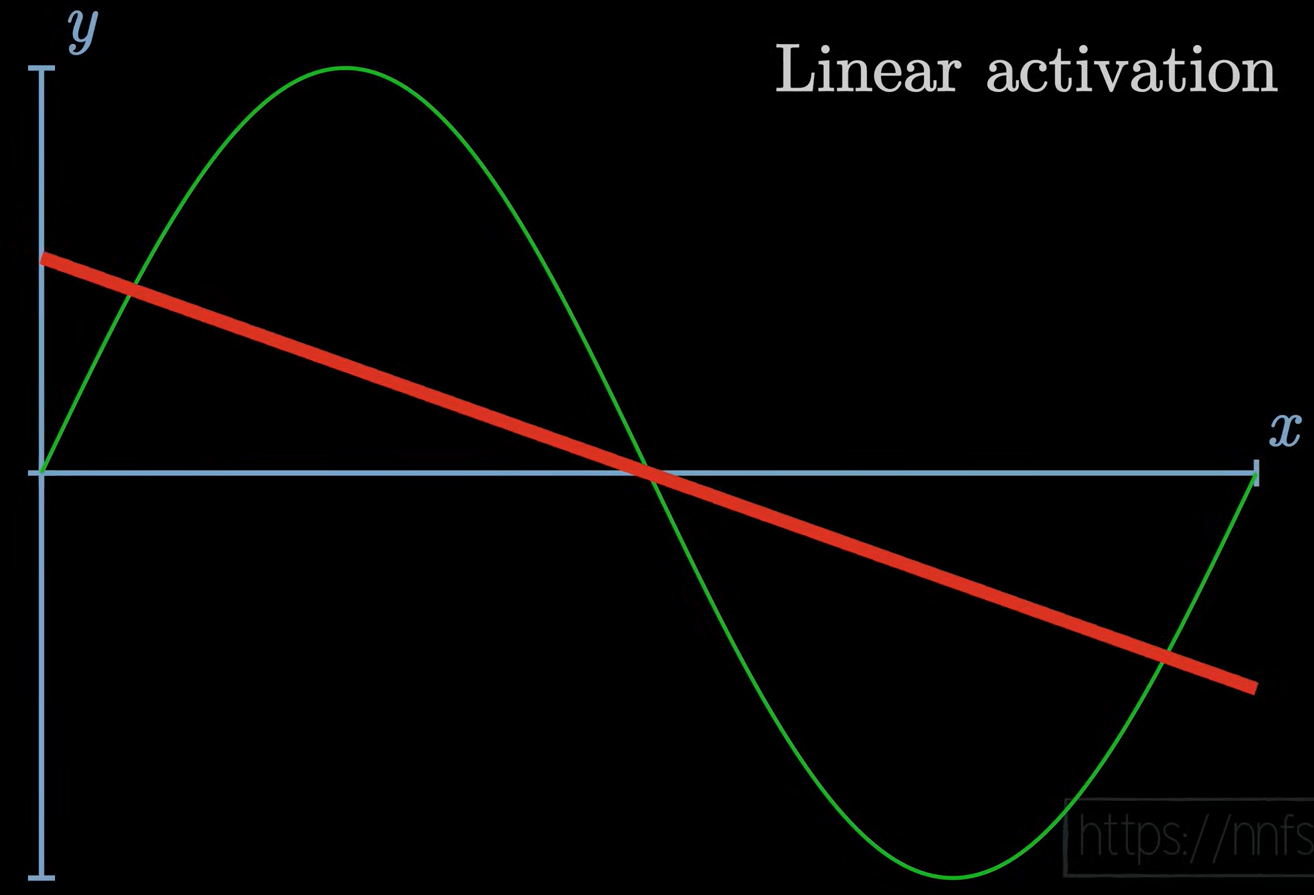
\includegraphics[width=0.5\textwidth]{Linear Activation.png} % width is in fraction of textwidth
    % \caption{Sample Image}% Caption of the image
    \label{fig:veri1}
\end{figure}

\subsection{Backpropagation}

Reference: \href{https://youtu.be/dB-u77Y5a6A?si=pFKasZnTR1_GaS5v}{Lecture by Justin Johnson}

\section{PyTorch}

Reference: \href{https://youtube.com/playlist?list=PLKnIA16_Rmvboy8bmDCjwNHgTaYH2puK7&si=q46c4wbwDzqZEilV}{Deep Learning using PyTorch - YouTube Playlist} 

\vspace{1em}

In 2002, Torch was a scientific computing framework with wide support for machine learning algorithms. 
But there were two problems in Torch: first, it is written in Lua, which is not widely used in the industry; second, it was using the static computational graph, which is not flexible and dynamic like PyTorch/ TensorFlow.

\vspace{0.5em}

These problems are fixed by PyTorch which is an open-source machine learning library developed by Facebook's AI Research lab. It is widely used for deep learning applications and provides a flexible and dynamic computational graph, making it easy to build and train neural networks.

\vspace{0.5em}

Core Features of PyTorch include:
\begin{itemize}[nosep]
    \item \textbf{Tensor Computations:} PyTorch provides a multi-dimensional array (tensor) library that is similar to NumPy but with GPU acceleration.
    \item \textbf{GPU Acceleration:} PyTorch can utilize GPUs for faster computation, making it suitable for deep learning tasks.
    \item \textbf{Dynamic Computation Graph:} PyTorch uses a dynamic computation graph, allowing for more flexibility in building and modifying neural networks.
    \item \textbf{Automatic Differentiation:} PyTorch uses a technique called automatic differentiation to compute gradients for high optimization tasks.
    \item \textbf{Distributed Training:} Training models on multiple GPUs or across multiple machines rather than a single GPU.
    \item \textbf{Interoperability with other libraries:} PyTorch can easily integrate with other popular libraries such as NumPy, SciPy, and Cython.
\end{itemize}

\subsection{What are Tensors?}

Tensors are a fundamental data structure in PyTorch, representing multi-dimensional arrays. They are similar to NumPy arrays but with additional capabilities for GPU acceleration and automatic differentiation. Tensors can be created from Python lists or NumPy arrays and can be manipulated using a variety of operations.

\vspace{0.5em}

\textbf{Examples:}
\begin{itemize}[itemsep=0.1em]
    \item \textbf{0D Tensor (Scalar):} A scalar tensor is a single value, which can be created from a Python number or a NumPy scalar. Output of Loss function is a scalar value.
    \item \textbf{1D Tensor:} A 1D tensor is an array or vector, which can be created from a Python list or NumPy array. The feauture vector of text is a 1D tensor, also known as embedding vector.
    \item \textbf{2D Tensor:} A 2D tensor is a matrix, which can be created from a list of lists or a 2D NumPy array. Gray Scale images are 2D tensors, where each pixel is represented by a single value like MNIST dataset.
    \item \textbf{3D Tensor:} A 3D tensor is a cube, which can be created from a list of 2D arrays or a 3D NumPy array. RGB images are 3D tensors, where each pixel is represented by three values (R, G, B).
    \item \textbf{4D Tensor:} A 4D tensor is a hypercube, which can be created from a list of 3D arrays or a 4D NumPy array. Video frames or Batch of RGB images are 4D tensors, where each frame is represented by a 3D tensor (RGB image).
    \item \textbf{5D Tensor:} Video data can be represented as a 5D tensor, where each frame is a 3D tensor (RGB image) and the batch size is the first dimension. For example, a batch of 10 video clips, each with 30 frames, can be represented as a 5D tensor with shape (10, 30, height, width, 3 RGB channels).
\end{itemize}

\subsection{Concept of seeding}

Seeding is a technique used to ensure that the random number generation in PyTorch is reproducible. By setting a seed value, we can ensure that the same random numbers are generated each time we run the code, which is useful for debugging and testing purposes.
A seed is a number that initializes the random number generator. If you use the same seed, you'll get the same sequence of random numbers.

\begin{center}
\begin{tabular}{|l|p{0.5\textwidth}|}
\hline
\textbf{Function} & \textbf{Purpose} \\
\hline
\texttt{torch.manual\_seed(seed)} & Sets the seed for \textbf{CPU} random number generation in PyTorch. \\
\hline
\texttt{torch.cuda.manual\_seed(seed)} & Sets the seed for \textbf{current GPU}. \\
\hline
\texttt{torch.cuda.manual\_seed\_all(seed)} & Sets the seed for \textbf{all GPUs}. \\
\hline
\texttt{torch.backends.cudnn.deterministic = True} & Forces cuDNN to use deterministic algorithms (slower, but reproducible). \\
\hline
\texttt{torch.backends.cudnn.benchmark = False} & Disables the auto-tuner that may introduce non-determinism. \\
\hline
\end{tabular}
\end{center}

\subsection{Autograd}

Autograd is PyTorch's automatic differentiation engine that powers neural network training. It allows us to compute gradients automatically, which is essential for optimizing model parameters during training.

Autograd keeps a record of data (tensors) and all executed operations in a directed acyclic graph (DAG) consisting of Function objects. \ul{For DAG, leaves are the input tensors, and roots are the output tensors}. By traversing this graph in reverse (backpropagation), we can compute gradients for all tensors involved in the computation.

\vspace{1em}

In a forward pass, autograd does two things simultaneously: \\
• run the requested operation to compute a resulting tensor\\
• maintain the operation's gradient function in the DAG.

\vspace{0.5em}

The backward pass kicks off when . backward() is called on the DAG root. autograd then:\\
• computes the gradients from each .grad\_fn ,\\
• accumulates them in the respective tensor's . grad attribute \\
• using the chain rule, propagates all the way to the leaf tensors.

\vspace{1em}

\textbf{Clearing Gradients}

After the backward pass, it's important to clear the gradients of the model parameters to prevent accumulation from previous iterations. This is typically done using the following command:

\begin{verbatim}
{Leaf(input)_Variable_Name}.grad.zero_()
\end{verbatim}

The Underscore after zero indicates that the operation is done in-place. 

There is other command \texttt{optimizer.zero\_grad()} which is used to clear the gradients of all model parameters in a single call. This is often used in training loops to reset gradients before the next forward and backward pass.
This function sets the gradients of all model parameters to zero, ensuring that the next forward and backward pass starts with a clean slate.

\vspace{1em}

\textbf{Stopping the Backpropagation}

After the model is trained, we may want to stop the backpropagation for certain tensors/operations. This can be done in three ways:

\begin{itemize}[nosep]
    \item \texttt{detach()} - Returns a new tensor that shares the same data but does not require gradients. This is useful when we want to use a tensor in a computation without tracking its gradients.
    \item \texttt{with torch.no\_grad():} - A context manager that temporarily disables gradient tracking. This is useful for inference or evaluation, where we don't need to compute gradients.
    \item \texttt{requires\_grad=False} - Setting this attribute on a tensor prevents it from being included in the computation graph and stops gradient tracking for that tensor.
\end{itemize}

% example
\begin{lstlisting}[language=Python]
import torch
# Create a tensor with requires_grad=True
x = torch.tensor([1.0, 2.0, 3.0], requires_grad=True)
# Perform some operations
y = x * 2 + 1
# Compute gradients
y.backward(torch.tensor([1.0, 1.0, 1.0]))  # Backpropagate
print(x.grad)  # Print gradients
# Detach the tensor from the computation graph
x_detached = x.detach()  # Detach x from the graph
# Perform operations without tracking gradients
y_no_grad = x_detached * 2 + 1  # No gradients will be computed
# Use with torch.no_grad() context
with torch.no_grad():
    y_no_grad = x * 2 + 1  # No gradients will be computed
# Set requires_grad=False
x.requires_grad = False  # Stop tracking gradients for x
\end{lstlisting}

\subsection{Training a Basic Neural Network}
\href{https://youtu.be/MKxEbbKpL5Q?si=rq2xCbflcuIfhI3e}{Youtube Video by CampusX}

Here, we are discussing few important points discussed in the video above, which is a good introduction to training a basic neural network using PyTorch.
Following are the steps to train a basic neural network using PyTorch:

\subsubsection{Import Required Libraries}

\subsubsection{Pre-Processing the Data}

Before training a neural network, we need to prepare the data. This involves loading the dataset, preprocessing it, and splitting it into training and validation sets. PyTorch provides several utilities for data loading and preprocessing, such as the \texttt{torchvision} library for image datasets.

\vspace{0.5em}

The data values should be normalized to a range of 0 to 1 or -1 to 1, depending on the activation function used in the neural network. This helps in faster convergence during training.

We use methods from scikit learn for data scaling, such as \texttt{StandardScaler} for standardization. 

\begin{lstlisting}[
    language=Python,
    backgroundcolor={\color{gray!10}},
    numbers = none,
]
  from sklearn.preprocessing import StandardScaler

  # Create a StandardScaler object
  scaler = StandardScaler()

  # Fit the scaler on the training data
  scaler.fit(X_train)

  # Transform the training and validation data
  X_train_scaled = scaler.transform(X_train)
  X_val_scaled = scaler.transform(X_val)
  # Note: Do not fit the scaler on validation data, only transform it.

  # Convert the scaled data to PyTorch tensors
  X_train_tensor = torch.tensor(X_train_scaled, dtype=torch.float32)
  X_val_tensor = torch.tensor(X_val_scaled, dtype=torch.float32)

  # Convert the labels to PyTorch tensors
  y_train_tensor = torch.tensor(y_train, dtype=torch.long)
  y_val_tensor = torch.tensor(y_val, dtype=torch.long)
\end{lstlisting}

While normalizing the data, keep in mind to use the same normalization parameters statistics (mean and standard deviation) for both training and validation datasets. This ensures that the model sees the same scale of data during both training and evaluation. This is done by using the \texttt{fit} method on the training data and then using the \texttt{transform} method on both training and validation data as shown in above code snippet.

\subsubsection{Define the Neural Network}

\subsubsection{Writing Training Pipeline}

From the Autograd section, we know that we need to compute the gradients of the loss function with respect to the model parameters. This is done using the \texttt{backward()} method on the loss tensor as shown below:

\begin{verbatim}
loss.backward()
\end{verbatim}

This loss can be computed using a loss function which we can get from the \texttt{torch.nn} module or can be defined explicitly in Neural Network class. 

There are two things we have to keep in mind, 

\begin{itemize}
    \item To make the gradients zero before the backward pass, we need to call the \texttt{zero\_grad()} method on the model parameters. This is important because PyTorch accumulates gradients by default, and we want to avoid accumulating gradients from previous iterations.
    \item To turn off the gradient tracking for the model parameters while updating the parameters or running the models for evaluation, we can use the \texttt{torch.no\_grad()} context manager or this is handled by the optimizer itself while using \texttt{optimizer.step()}.
\end{itemize}

\subsubsection{Evaluation}

\subsubsection{Basics of OOPS in Python}

Reference: \href{https://www.youtube.com/watch?v=HQnoYzxOHMw}{Video-1} (Intro to OOPS) \href{https://youtu.be/a7baAGCBA9U?si=dic4GqzG0pJtPffX}{Video-2} (Classes \& Objects) \href{https://youtu.be/12HRkYld22c?si=2YsB6D_8Efi1Otr0}{Video-3} (Constructors) \href{https://youtu.be/6soT3DMBJGQ?si=9a_6DyX1GmZFHFg9}{Video-4} (Inheritance) 

\vspace{0.5em}

Coding Neural Networks in PyTorch involves defining classes, objects and methods. This also includes concept related to inheritance, polymorphism, and encapsulation. So, its good to go through the above videos to understand the basics of OOPS in Python.

\subsection{Using NN Pytorch Module}
The \texttt{torch.nn} module in PyTorch provides a high-level interface for building neural networks. It includes pre-defined layers, loss functions, and optimizers that make it easier to construct and train neural networks.
Key components of torch.nn include:
\begin{itemize}[nosep]
    \item \textbf{Modules:} The \texttt{nn.Module} class is the base class for all neural network modules in PyTorch. It provides methods for defining the forward pass and managing parameters.
    \item \textbf{Layers:} Pre-defined layers like \texttt{nn.Linear}, \texttt{nn.Conv2d}, and \texttt{nn.ReLU} for building neural networks.
    \item \textbf{Activation Functions:} Pre-defined activation functions like \texttt{nn.ReLU}, \texttt{nn.Sigmoid}, and \texttt{nn.Tanh} for introducing non-linearity in the network, allowing it to learn complex patterns.
    \item \textbf{Loss Functions:} Pre-defined loss functions like \texttt{nn.CrossEntropyLoss} and \texttt{nn.MSELoss} for computing the loss during training.
    \item \textbf{Sequential:} The \texttt{nn.Sequential} class allows us to define a neural network as a sequence of layers, making it easier to build simple feedforward networks.
    \item \textbf{Optimizers:} Pre-defined optimizers like \texttt{torch.optim.SGD} and \texttt{torch.optim.Adam} for updating model parameters during training.
    \item \textbf{Dropout and Batch Normalization:} Layers like \texttt{nn.Dropout} and \texttt{nn.BatchNorm2d} for regularization and normalization. The \texttt{nn.Dropout} layer is used to prevent overfitting by randomly setting a fraction of input units to zero during training.
\end{itemize}

\subsection{Dataset \& DataLoader Class}

There are the following problems with the traditional way of loading data in PyTorch:
\begin{itemize}
    \item Loading the entire dataset into memory at once can be inefficient and may not fit into memory for large datasets.
    \item Data augmentation techniques like random cropping, flipping, and rotation are often needed to improve model generalization.
    \item Shuffling the dataset is important to ensure that the model does not learn any unintended patterns from the order of the data.
    \item Batching the data with efficient parallelism is necessary to speed up training and make better use of hardware resources.
\end{itemize}

These problems are addressed by the Dataset and DataLoader classes in PyTorch. The Dataset class is an abstract class that represents a dataset and provides methods for accessing individual data samples. The DataLoader class is responsible for loading data from a Dataset and providing it in batches, with support for shuffling, parallel loading, and data augmentation.

\subsubsection{Dataset Class}

The Dataset class is essentially a blueprint. When we create a custom Dataset, we decide how data is loaded and returned. It defines:

\vspace{-0.6em}

\begin{itemize}[itemsep=0.1em]
    \item \texttt{\_\_init\_\_()} method: Initializes the dataset, loads data from files, and performs any necessary preprocessing.
    \item \texttt{\_\_len\_\_()} method: Returns the total number of samples in the dataset.
    \item \texttt{\_\_getitem\_\_(index)} method: Returns a single sample from the dataset at the specified index. This is where we can apply data transformations or augmentations.
\end{itemize}

\begin{lstlisting}[
    language=Python,
    backgroundcolor={\color{gray!10}},
    numbers=none,
    % nolol=true,
]
import torch
from torch.utils.data import Dataset

class CustomDataset(Dataset):
    def __init__(self, data, labels, transform=None):
        self.data = data
        self.labels = labels
        self.transform = transform

    def __len__(self):
        return self.data.shape[0]  # Return the total number of samples

    def __getitem__(self, index):
        sample = self.data[index]
        label = self.labels[index]
        if self.transform:
            sample = self.transform(sample) # Apply any transformations if provided
        return sample, label
\end{lstlisting}

Here, \texttt{data} is the input and \texttt{labels} are the corresponding labels/Output for the input data. The \texttt{transform} parameter is optional and can be used to apply any transformations to the data samples, such as normalization or data augmentation.

\subsubsection{DataLoader Class}

The DataLoader class is responsible for loading data from a Dataset and providing it in batches. 
At the start of each epoch, the DataLoader (if shuffle-True) shuffles indices(using a sampler). It divides the indices into chunks of batch size. for each index in the chunk, data samples are fetched from the Dataset object The samples are then collected and combined into a batch (using collate\_fn). The batch is returned to the main training loop.

We don't need to write class for DataLoader, as it is already provided by PyTorch. We can use it directly to load data from our custom Dataset as following:

\begin{lstlisting}[
    language=Python,
    backgroundcolor={\color{gray!10}},
    numbers=none,
    % nolol=true,
]
from torch.utils.data import DataLoader
    # Create an instance of the custom dataset
    dataset = CustomDataset(data, labels, transform=transform)

    # Create a DataLoader instance
    dataloader = DataLoader(dataset, batch_size=32, shuffle=True, num_workers=4)

    for epoch in range(num_epochs):
        # Iterate through the DataLoader
        for batch_data, batch_labels in dataloader:
            # Perform training or evaluation on the batch
            pass
\end{lstlisting}

\section{RISC-V}

RISC-V is an open standard instruction set architecture (ISA) based on established reduced instruction set computer (RISC) principles. The specification for this set of instructions is the 5th generation of RISC processors, which have been in development since the 1980s, thus we call it RISC-V. RISC-V ecosystem consists of following elements:
\begin{itemize}
    \item Physical hardware: Processors, development boards, System-on-Chips (SoCs), System-on-Modules (SoMs), and other physical systems.
    \item ``Soft'' IP processor cores that can be loaded into emulators, field-programmable gate arrays (FPGAs), or implemented in silicon.
    \item The entire software stack, from bootloaders and firmware, up to full operating systems and applications.
    \item Educational material including courseware, curricula, lesson plans, online courses like this one, tutorials, podcasts, lab assignments, and even books.
    \item Services including verification, custom board design, and many more.
\end{itemize} 

\subsection{RISC vs. CISC: Instruction Sets and Code Density}
RISC-V follows the RISC (Reduced Instruction Set Computer) philosophy, which contrasts with the CISC (Complex Instruction Set Computer) approach used in architectures like x86. A key distinction between these approaches involves two separate concepts that are often confused:

\begin{itemize}
    \item \textbf{Instruction Set Size}: The number of unique instruction types defined by the architecture
    \item \textbf{Instruction Count in Programs}: The number of instruction instances needed to implement a specific task
\end{itemize}

CISC architectures typically have \ul{\textit{larger} instruction sets (more unique instructions)} where \ul{most of which have access to memory} but require \ul{\textit{fewer} instructions to implement} a given program. For example, Intel's 80386 introduced in 1985 supported over 150 distinct instructions.

In contrast, RISC architectures like RISC-V have \ul{\textit{smaller} instruction sets (fewer unique instructions)} with \ul{memory access restricted to a few Load and Store instructions} but may require \ul{\textit{more} instructions to implement the same functionality}. The RISC-V base integer instruction set includes only 40 instructions.

\vspace{1em}
To illustrate this difference, consider a simple operation of adding a value from memory to a register:

\begin{center}
\begin{tabular}{|l|l|}
\hline
\textbf{CISC Approach} & \textbf{RISC Approach} \\
\hline
\texttt{ADD REG, [ADDR]} & \texttt{LOAD REG2, [ADDR]} \\
(One instruction) & \texttt{ADD REG1, REG1, REG2} \\
 & (Two instructions) \\
\hline
\end{tabular}
\end{center}

\vspace{1em}
This design choice in RISC architectures enables simpler hardware implementations, more efficient pipelining, and often better performance despite requiring more instructions to accomplish the same tasks. The tradeoff of using more, simpler instructions instead of fewer, complex instructions has proven beneficial for most modern processor designs.

Prof. Krste Asanović and graduate students Yunsup Lee and Andrew Waterman started the RISC-V instruction set in May 2010 as part of the Parallel Computing Laboratory (Par Lab) at UC Berkeley, of which Prof. David Patterson was Director. The Par Lab was a five-year project to advance parallel computing funded by Intel and Microsoft for \$10M over 5 years, from 2008 to 2013.

\subsection{RISC-V Name}
The name RISC-V was chosen to represent the fifth major RISC ISA design from UC Berkeley (RISC-I [15], RISC-II [8], SOAR [21], and SPUR [11] were the first four). We also pun on the use of the Roman numeral “V” to signify “variations” and “vectors”, as support for a range of architecture research, including various data-parallel accelerators, is an explicit goal of the ISA design.

\subsection{RISC-V Instruction Set Variants}
RISC-V is not just one instruction set, but a family of related ISAs. The core part of each ISA is called a base integer instruction set, and there are currently four main versions:

\begin{itemize}[nosep]
    \item \textbf{RV32I} – 32-bit registers and address space (XLEN = 32)
    \item \textbf{RV64I} – 64-bit registers and address space (XLEN = 64)
    \item \textbf{RV32E} – A smaller version of RV32I, with only 16 integer registers (instead of 32), made for small microcontrollers
    \item \textbf{RV128I} – A future version with 128-bit registers and address space (XLEN = 128)
\end{itemize}

All these versions use two's-complement to represent signed integers.
XLEN is the term used to refer to the register width (32, 64, or 128 bits).

\subsection{Shakti Processors}
Resources: \url{https://en.wikipedia.org/wiki/SHAKTI_(microprocessor)} \\
\url{https://github.com/platformio/platform-shakti} \\

Shakti is an Indian-developed, open-source RISC-V processor started as an academic initiative back in 2014 by the Reconfigurable Intelligent Systems Engineering (RISE) group at IIT-Madras. 

\subsubsection{Shakti Processor Variants}
The Shakti processor family includes several variants, each designed for different applications and performance levels. The variants are categorized into classes based on their intended use:
\begin{center}
\begin{tabular}{|l|p{0.7\textwidth}|}
\hline
\textbf{Variant} & \textbf{Description} \\
\hline
\textbf{E-class} & Embedded microcontroller class (RV32IMA), no MMU \\
\hline
\textbf{C-class} & Controller-class (with MMU), runs Linux \\
\hline
\textbf{I-class} & Industrial-class, superscalar \\
\hline
\textbf{M-class} & Multicore high-performance \\
\hline
\textbf{S-class} & Server-grade \\
\hline
\textbf{H-class} & High-performance, out-of-order execution \\
\hline
\end{tabular}
\end{center}

There are experimental variants as well, such as the Shakti H-class, which is a high-performance processor with out-of-order execution capabilities.


\subsection{Vega Processors}
Resources: \url{https://en.wikipedia.org/wiki/VEGA_Microprocessors} \\

Vega processors are developed by the Centre for Development of Advanced Computing (C-DAC) in India.
% Vega is India's first indigenous 64-bit Multi-core RISC-V based Superscalar Out-of-Order Processor

An out-of-order processor is a type of processor that executes instructions in a different order than they are written in the program, as long as it maintains the correct order of execution to ensure the program works correctly.
\subsubsection{Vega Processor Variants}
The Vega processor family includes several variants:

\begin{center}
\begin{tabular}{|l|p{0.7\textwidth}|}
\hline
\textbf{Variant} & \textbf{Description} \\
\hline
\textbf{Vega ET1031} & Embedded 32-bit processor with floating-point unit (FPU) support \\
\hline
\textbf{Vega ET1040} & Higher performance variant with memory management unit (MMU) \\
\hline
\textbf{Vega AS1061} & Security-focused variant with enhanced protection features \\
\hline
\end{tabular}
\end{center}

The Vega Series is entirely open-source and compatible with multiple toolchains, making it flexible for various development environments.

\section{SystemVerilog}

Refer: \href{https://youtube.com/playlist?list=PLqPfWwayuBvMwUjNHfyaX6CTK2KbeL2ga&si=NyddrPqUN_h-WrtD}{Youtube Playlist}\\
EDA Playground Link for Practicing : \url{https://edaplayground.com/x/t7M2}

Drawback of Verilog: Not able to extensively verify the design. Missing the Corner Cases

\subsection{About RTL}

Refer: \href{https://www.reddit.com/r/vlsi_enthusiast/comments/1ffoqd4/what_is_rtl_register_transfer_level_design_in_vlsi/}{Reddit Post}\\ 

RTL stands for Register Transfer Level, which is a design abstraction used in digital circuit design. The above Reddit post link gives the detailed RTL description, its uses and importance in VLSI design.

\subsection{Verilog Vs SystemVerilog}

Refer: \href{https://www.reddit.com/r/Verilog/comments/oqkcj5/difference_between_verilog_and_system_verilog/}{Reddit Post}\\ 

Verilog is subset of SystemVerilog. SystemVerilog is an extension of Verilog that includes additional features and capabilities, particularly for verification and design abstraction. Refer the above Reddit post for more details.\\

Think of SystemVerilog as C++ and Verilog as C. Everything you can write in C will work in C++, but C++ offers much more.\\

Vanilla Verilog is the pure, standard Verilog — without any SystemVerilog features. When someone says "vanilla Verilog", they usually mean "just Verilog, no SystemVerilog".


\subsection{Data Types}
Recalling for the data types in Verilog, we have reg, wire, integer, time, real etc. All these are 4-state data types, meaning they can take values 0, 1, X (unknown), and Z (high impedance).

In case of SystemVerilog, we have the following data types:

\begin{center}
\begin{tabular}{|l|l|p{0.5\textwidth}|}
\hline
\textbf{Data Type} & \textbf{States} & \textbf{Description} \\
\hline
\texttt{logic} & 4-state & Can be used in both procedural and continuous assignments (one at a time) \\
\hline
\texttt{bit} & 2-state & Can only take values 0 or 1, more efficient for synthesis \\
\hline
\texttt{enum} & Variable & Enumerated data type allowing named constant values \\
\hline
\texttt{struct} & Variable & Composite data type grouping related variables \\
\hline
\texttt{typedef} & N/A & User-defined type declarations for code reusability \\
\hline
\end{tabular}
\end{center}

Values of \texttt{reg} can only be assigned in procedural blocks like \texttt{always}  and \texttt{initial} blocks, while \texttt{wire} can only be assigned in continuous assignments using assign statements. Sometimes, we get confused between what to use (\texttt{wire} or \texttt{reg}) when and where. So to avoid this confusion, we can use  \texttt{logic} data type in SystemVerilog, which can be used in both procedural and continuous assignments (one at a time).

\vspace{1em}

Defining a variable as \texttt{logic} will let us use it in either procedural blocks (like \texttt{always} or \texttt{initial}) or continuous assignments (like \texttt{assign} statements).

\textbf{Example Usage:}
\begin{lstlisting}[language=Verilog]
// SystemVerilog logic data type
logic [7:0] data_bus;    // Can be used flexibly
logic       clock;       // Single bit logic

// Traditional Verilog approach
reg  [7:0] data_reg;     // Only in procedural blocks  
wire [7:0] data_wire;    // Only in continuous assignments
\end{lstlisting}

default value of both \texttt{reg} and \texttt{logic} is \texttt{X} (unknown) in simulation.

\subsubsection{2-State Data Types}
These data types can only take values 0 or 1, making them more efficient for synthesis and simulation. Following are the 2-state data types in SystemVerilog:

\begin{center}
\begin{tabular}{|l|p{0.7\textwidth}|}
\hline
\textbf{Data Type} & \textbf{Description} \\
\hline
\texttt{bit} & Unsigned single bit data type that can take values 0 or 1. \\
\hline
\texttt{byte} & An 8-bit signed data type that can take values from -128 to 127. It is a convenient way to represent small integers. \\
\hline
\texttt{shortint} & A 16-bit signed integer data type that can take values from -32768 to 32767. It is useful for representing small signed integers. \\
\hline
\texttt{int} & A 32-bit signed integer data type that can take values from -2147483648 to 2147483647. It is the default integer type in SystemVerilog. \\
\hline
\texttt{longint} & A 64-bit signed integer data type that can take values from -9223372036854775808 to 9223372036854775807. It is useful for representing large signed integers. \\
\hline
\end{tabular}
\end{center}

\textbf{Important Note:} What will happen if we assign x or z to these 2-state data types?

If x or z values are assigned to 2-state data types, then it will be automatically converted to 0.

\subsubsection{Struct Data Type}
The difference between \texttt{struct} and \texttt{array}
is that grouping of different data types in \texttt{struct} while \texttt{array} is grouping of same data types.

\vspace{1em}
Following is the syntax for defining a struct in SystemVerilog:

\begin{lstlisting}[
    language=Verilog,
    backgroundcolor={\color{gray!10}},
    numbers =none,
    % nolol=true
    ]
    // SystemVerilog struct data type
    struct packed {
        logic [7:0] data;  // 8-bit data field
        logic valid;       // Validity flag
    } my_struct;          // Instance of the struct

    // Accessing struct fields
    my_struct.data = 8'hFF;  // Assigning value to data field
    my_struct.valid = 1'b1;  // Assigning value to valid field
    // Using struct in a module
\end{lstlisting}

\textbf{Packed vs Unpacked Structs:}

Above code defines a \textit{packed} struct in SystemVerilog. 

Packed structs are stored in a contiguous block of memory, with no padding between fields. This makes them more efficient for hardware representation. Good for synthesizable code or bit-level operations.

\vspace{1em}

Unpacked structs, on the other hand, allow for padding and can have variable-sized fields. They are more flexible but less efficient for hardware representation. Each member may be separately stored.

\begin{lstlisting}[
    language=Verilog,
    backgroundcolor={\color{gray!10}},
    numbers =none,
    % nolol=true,
    title={Packed vs Unpacked Structs}
]
    typedef struct packed {           |     typedef struct {
      logic [3:0] a;                  |       logic [3:0] a;
      logic [3:0] b;                  |       logic [3:0] b;
    } my_struct_t;                    |     } my_struct_t;
    +----------+----------+
    | bits 7:4 | bits 3:0 |
    |    a      |    b      |
    +----------+----------+
\end{lstlisting}

\vspace{1em}

\textbf{Using Typedef}

Typedef allows us to create new data types based on existing ones. This can help improve code readability and maintainability by giving meaningful names to complex data types.


\begin{lstlisting}[
    language=Verilog,
    backgroundcolor={\color{gray!10}},
    numbers =none,
    % nolol=true,
    title={Verilog Code using Typedef}
    ]
    logic [7:0] byte_t;               |     typedef logic [7:0] byte_t;  
    // Here, byte_t is a variable     |     // Define a new type byte_t
    logic [7:0] data1;                |     byte_t data1;     
    logic [7:0] data1;                |     byte_t data2;   
                                      |     // variables of type byte_t
\end{lstlisting}


\textbf{Good Example}

\begin{lstlisting}[
    language=Verilog,
    backgroundcolor={\color{gray!10}},
    numbers =none,
    % nolol=true,
    title={Good Example of Packed Struct Usage with Typedef}
]
    typedef struct packed {
        logic [3:0] a;
        logic [3:0] b;
    } my_struct_t;

    my_struct_t s;
    initial begin
    s = 8'b10001100; // assign whole struct as 8-bit value
    end
\end{lstlisting}

In the above example, the packed struct \texttt{my\_struct\_t} is defined with two 4-bit fields \texttt{a} and \texttt{b}. The struct can be assigned a single 8-bit value where first four bits correspond to \texttt{a} and the last four bits correspond to \texttt{b}. So here, a= 1000 (8) and b=1100 (12).

\vspace{1em}

\subsubsection{Enumerated Data Types}

Enumerated data types allow us to define a set of named values, which can make our code more readable and maintainable. They are particularly useful for representing states or modes in our design.

\begin{lstlisting}[
    language=Verilog,
    backgroundcolor={\color{gray!10}},
    numbers =none,
    % nolol=true,
    title={Enumerated Data Type Example}
]
    typedef enum {IDLE, RUNNING, DONE} state_t; // Define an enumerated type
    state_t current_state; // Declare a variable of the enumerated type
    // current state is a variable of enum data type which can take values IDLE, RUNNING, or DONE
    initial begin
        current_state = IDLE; // Assign a named value to the variable
    end
\end{lstlisting}

\subsubsection{Fixed Arrays (Packed/Unpacked)}

Arrays in SystemVerilog can be one-dimensional or multi-dimensional, and they can be packed or unpacked. Packed arrays are stored in a contiguous block of memory, while unpacked arrays allow for variable-sized elements. 

Packed arrays are typically used when you need to manipulate the entire array as a single unit at bit level operations, particularly for tasks like bit slicing or packing/unpacking data.

\textbf{Note:} Packed arrays have restrictions on the data types they can use. We cannot use the 2-state data types like \texttt{int}, \texttt{byte}, \texttt{shortint}, or \texttt{longint} with packed arrays. \ul{Packed arrays can only be used with data types like \texttt{logic}, \texttt{bit}, and \texttt{enum}.}

\vspace{1em}

\textbf{Example of Packed Array:} 
Following is the syntax for one-dimensional two bit packed array:
\begin{lstlisting}[
    backgroundcolor={\color{grey}},
    frame= none,
    numbers=none,
    xleftmargin=.35\textwidth,
    xrightmargin=.3\textwidth, 
    ]
    bit [1:0] array;
\end{lstlisting}

\textbf{Note:} Here, we don't need to use the keyword \texttt{packed} explicitly like we did for structs.

\vspace{0.5em}
For multi-dimensional packed arrays, the data will be stored in contiguous memory locations only like in linear one dimensional fashion. The syntax for a two-dimensional packed array is as follows:

\begin{lstlisting}[
    backgroundcolor={\color{grey}},
    frame= none,
    numbers=none,
    xleftmargin=.35\textwidth,
    xrightmargin=.3\textwidth, 
    ]
    bit [1:0][2:0] array;
\end{lstlisting}

In unpacked arrays, the \ul{ array dimensions are mentioned after the variable name} and they \ul{can be of any data type} like \texttt{int}, \texttt{byte}, \texttt{shortint}, or \texttt{longint}.

\vspace{1em}

\textbf{Example of Unpacked Array:}
\begin{lstlisting}[
    backgroundcolor={\color{grey}},
    frame= none,
    numbers=none,
    xleftmargin=.35\textwidth,
    xrightmargin=.3\textwidth, 
    ]
    int array [1:0][2:0]; 
\end{lstlisting}

This defines a two-dimensional unpacked array where the first dimension has 2 elements and the second dimension has 3 elements. The data type of the elements is \texttt{int}.

\begin{lstlisting}[
    backgroundcolor={\color{grey}},
    frame= none,
    numbers=none,
    xleftmargin=.3\textwidth,
    xrightmargin=.25\textwidth, 
    ]
    bit [1:0] packed_array [3:0];
\end{lstlisting}

Here, we have defined a packed array named \texttt{packed\_array} with 4 elements, each of which is 2 bits wide. The elements can be accessed using indices like \texttt{packed\_array[0]}, \texttt{packed\_array[1]}, etc. It is packed along one dimension that is [1:0] is continuous memory locations but unpacked along the other dimension that is [3:0] is not continuous memory locations.

\textbf{Assigning Values to Arrays:}
\begin{lstlisting}[
    language=Verilog,
    backgroundcolor={\color{gray!10}},
    numbers =none,
    % nolol=true,
    title={Assigning Values to Array}
]
    int unpacked_array [3:0];           |    int unpacked_array [3:0];
    // 4 int elements                   |
    packed_array[0] = 2'b01;            |
    packed_array[1] = 2'b10;            |   unpacked_array = '{10,20,30,40};
    packed_array[2] = 2'b11;            |   // Use ' to assign values 
    packed_array[3] = 2'b00;            |   // directly to the entire array
\end{lstlisting}


In the above example, using apostrophe (') allows us to assign values directly to the entire array in one go. This is particularly useful for initializing arrays with known values. This will give unpacked\_array[0] = 40 unpacked\_array[1] = 30 and so on.

\vspace{1em}

\textbf{Accessing Array Elements:}

To access all elements of an array, we can use a \texttt{foreach} loop in SystemVerilog. This loop iterates over each element of the array, allowing us to perform operations on them. This is similar to the \texttt{for} loop in C/C++. We can also use \texttt{for} loop to access the elements of the array.
\begin{lstlisting}[
    language=Verilog,
    backgroundcolor={\color{gray!10}},
    numbers =none,
    % nolol=true,
    title={Accessing Array Elements using foreach}
]
    foreach (packed_array[i]) begin
        // Access each element of packed_array
        $display("Element %0d: %b", i, packed_array[i]);
    end

    // Using for loop to access elements
    for (int i = 0; i < $size(packed_array); i++) begin
        $display("Element %0d: %b", i, packed_array[i]);
    end
\end{lstlisting}

\textbf{Note:} The \texttt{foreach} loop is particularly useful for iterating over arrays with dynamic sizes, as it automatically adjusts to the size of the array.

\vspace{0.5em}

\textbf{Packed Array Example:}
\begin{lstlisting}[
    language=Verilog,
    backgroundcolor={\color{gray!10}},
    numbers =none,
    title={Packed Array Example}
]
module example;
    bit [2:0][3:0][7:0] data; 

    initial 
        begin
            data = 96'hffff_ffff_ffef_ffef_aaaa_aaaa_bbbb_bbbb;
            $display("the value of data is: %b", data);
            
            // Display array values
            foreach (data[i]) 
                begin
                    $display("data[%0d] = %b", i, data[i]);
                foreach (data[i][j]) 
                    begin
                        $display("data[%0d][%0d] = %b", i, j, data[i][j]);
                    end
                end
        end
endmodule
\end{lstlisting}

\textbf{Output:}
\vspace{-0.5em}
\begin{figure}[H]
    \centering
    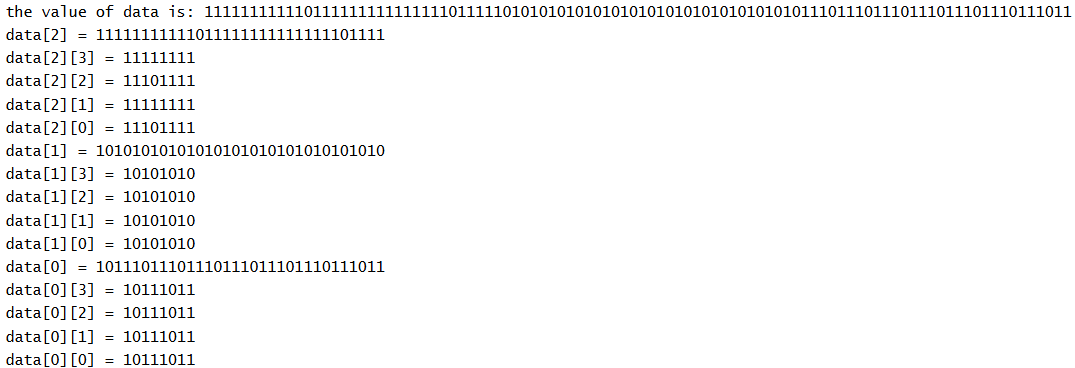
\includegraphics[width=1\textwidth]{Packed_Output.png}
\end{figure}

\subsubsection{Dynamic Arrays}

\textbf{Compile Time vs Runtime}

Compile-time refers to the phase in the development process when the source code is translated into machine code (or intermediate code) by a compiler. This phase happens before the program is run. The goal of compile-time activities is to check and transform the code so that it is ready for execution.

\vspace{0.5em}

In HDLs like SystemVerilog, compile-time refers to \ul{the time when the compiler checks for the syntax, and the HDL code is converted into a netlist} or hardware structure before execution of program.

\vspace{0.5em}

Runtime is the \ul{phase when the compiled code is executed on a computer or hardware}. During runtime, the program is running, and it can perform operations, access memory, produce output and interact with the user or other systems.

\vspace{1em}

Dynamic arrays are a type of array in SystemVerilog that can change size during simulation. They are particularly useful when the size of the array is not known at compile time and can be adjusted based on runtime conditions.

In case of Fixed Arrays, the size of the array is fixed at compile time, meaning it cannot be changed during runtime. Dynamic array do not have a fixed size at compile-time. The size is not known or set during compilation, and no memory is allocated for the array at this stage.

To declare a dynamic array, you use the following syntax:

\begin{lstlisting}[
    backgroundcolor={\color{grey}},
    frame= none,
    numbers=none,
    xleftmargin=.35\textwidth,
    xrightmargin=.3\textwidth, 
    ]
    int dynamic_array [];
\end{lstlisting}

In this example, we declare a dynamic array of integers. The size of the array can be set at runtime using the \texttt{new()} method:

\begin{lstlisting}[
    backgroundcolor={\color{grey}},
    frame= none,
    numbers=none,
    xleftmargin=.25\textwidth,
    xrightmargin=.2\textwidth, 
    ]
    dynamic_array = new[10]; // Create an array with 10 elements
\end{lstlisting}

Dynamic arrays can also be resized using the \texttt{resize()} method:

\begin{lstlisting}[
    backgroundcolor={\color{grey}},
    frame= none,
    numbers=none,
    xleftmargin=.25\textwidth,
    xrightmargin=.2\textwidth, 
    ]
    dynamic_array.resize(20); // Resize the array to 20 elements
\end{lstlisting}

\vspace{1em}
\textbf{Copying the elements of Dynamic Array:}

Without explicitly creating the memory for the second dynamic array, we can copy the elements of one dynamic array to another just by using the following syntax:
\begin{lstlisting}[
    backgroundcolor={\color{grey}},
    frame= none,
    numbers=none,
    xleftmargin=.22\textwidth,
    xrightmargin=.17\textwidth, 
    ]
    int dynamic_array2[] = dynamic_array; 
    // Copy elements to another dynamic array
\end{lstlisting}

If we make any changes to \texttt{dynamic\_array}, it will not affect \texttt{dynamic\_array2}. SystemVerilog creates an independent copy of the array. Both arrays will have separate memory locations, and changes to one array will not affect the other.

\vspace{1em}

\textbf{Increasing the size of Dynamic Array:}

There are two methods to increase the size of a dynamic array in SystemVerilog:
\begin{itemize}
    \item The existing elements will be deleted and size will be increased.
    \item The existing elements will remain as it is and size will be increased.
\end{itemize}

\begin{lstlisting}[
    language=Verilog,
    backgroundcolor={\color{gray!10}},
    numbers =none,
    % nolol=true,
    title={Resizing Dynamic Array}
    ]
    dyn1 = new[20];                         | dyn1 = new[20](dyn1);
  // Existing elements will be deleted      | // Existing elements will remain
                                            | // Size of dyn1 will be increased to 20
\end{lstlisting}

Lets say the initial size of dyn1 is 10, then after resizing it to 20, the first method will delete the existing 10 elements and create a new array of size 20. The second method will keep the existing 10 elements and increase the size to 20, leaving the last 10 elements uninitialized (default value is \texttt{0}).
\vspace{1em}

\textbf{Builtin  Functions for Dynamic Arrays:}
\begin{itemize}[nosep]
    \item \texttt{size()} - Returns the number of elements in the dynamic array.
    \item \texttt{delete()} - Deletes the dynamic array and frees up memory.
    \item \texttt{push\_back()} - Adds an element to the end of the dynamic array.
    \item \texttt{pop\_back()} - Removes the last element from the dynamic array.
\end{itemize}

\vspace{0.5em}

\href{https://vlsiverify.com/system-verilog/dynamic-array-in-sv/}{Here}
 is the link of good Dynamic Array example code.

\textbf{Dynamic Array Example:}



\subsubsection{Queue}
In SystemVerilog, a queue is a variable-size, ordered collection of homogeneous elements (all elements are of the same type). Unlike static arrays and dynamic arrays, the size of a queue can change dynamically during runtime as elements are added or removed. Queues provide a powerful, flexible data structure that operates like a FIFO (First In, First Out) or LIFO (Last In, First Out) mechanism depending on how you manipulate the elements.

\vspace{0.5em}

In dynamic arrays, we have to explicitly create the memory for the array using the \texttt{new()} method before inserting the elements, but in queues, we don't have to do that. Memory is allocated in the queue automatically when we add elements to them.

\textbf{Key Characteristics:}

\begin{itemize}[nosep]
    \item \textbf{Dynamic Size:} Queues can grow or shrink as needed as elements are deleted or inserted, allowing for flexible memory usage.

    \item \textbf{Operations:} Queues support various operations such as inserting, deleting elements to the front or back, and  querying the queue size.

    \item \textbf{Homogeneous Elements:} All elements in a queue must be of the same data type.
    \item \textbf{FIFO Behavior:} Elements are typically added to the end and removed from the front, following a first-in-first-out order.
\end{itemize}

Here is the general syntax for declaring a queue in SystemVerilog:
\begin{lstlisting}[
    backgroundcolor={\color{grey}},
    frame= none,
    numbers=none,
    xleftmargin=.3\textwidth,
    xrightmargin=.25\textwidth, 
    ]
    data_type queue_name [$];
\end{lstlisting}

For example, to declare a queue of integers, you would use:
\begin{lstlisting}[
    backgroundcolor={\color{grey}},
    frame= none,
    numbers=none,
    xleftmargin=.35\textwidth,
    xrightmargin=.3\textwidth, 
    ]
    int my_queue [$];
\end{lstlisting}
This creates a queue named \texttt{my\_queue} that can hold integers.

\textbf{Builtin Functions}

\vspace{0.2em}

\begin{itemize}[nosep]
    \item \texttt{size()} - Returns the number of elements in the queue.
    \item \texttt{insert(index, value)} - Inserts a value at the specified index in the queue.
    \item \texttt{delete(index)} - Deletes the value at specified index. In case if index is not mentioned, it deletes all elements in the queue and frees up memory.
    \item \texttt{push\_back(value)} - Adds an element to the end of the queue.
    \item \texttt{push\_front(value)} - Adds an element to the front of the queue.
    \item \texttt{pop\_front()} - Removes and returns the first element from the queue.
    \item \texttt{pop\_back()} - Removes and returns the last element from the queue.
\end{itemize}

\subsubsection{Associative Arrays}
As we have discussed earlier about dynamic arrays and fixed arrays, there we have allocate the fixed memory space either in the compile time or at the runtime irespective of the fact that we are using that memory or not. For example, if we declare a dynamic array of size 100, then 100 memory locations will be allocated for that array even if we are using only 10 elements in that array, remaining 90 elements are just waste of memory. 

\vspace{1em}

Associative arrays provide a way to store data where the index or key doesn't need to be an integer (can also be a string) and doesn't need to be consecutive, unlike dynamic arrays or fixed-size arrays. This makes them similar to dictionaries or maps in other programming languages. They are very useful when the index values are sparse or irregular, allowing flexible and dynamic data storage.

Following is the syntax for declaring an associative array in SystemVerilog:
\begin{lstlisting}[
    backgroundcolor={\color{grey}},
    frame= none,
    numbers=none,
    xleftmargin=.2\textwidth,
    xrightmargin=.15\textwidth, 
    ]
    data_type associative_array_name [key_type];
\end{lstlisting}

key\_type can be of any data type, including integers, strings, or enumerated types. \ul{* (Wildcard type) index type inferred at first use}.
data\_type is the data type of the elements stored in the associative array.

\vspace{0.5em}

For example, to declare an associative array of integers with string keys, you would use:
\begin{lstlisting}[
    backgroundcolor={\color{grey}},
    frame= none,
    numbers=none,
    xleftmargin=.13\textwidth,
    xrightmargin=.08\textwidth, 
    ]
module example;
    int marks[string];
    initial begin
        marks["Alice"] = 85;
        marks["Bob"] = 90;
        marks["Charlie"] = 78;
        
        $display("Alice's marks: %Od", marks["Alice"]);
        $display("Bob's marks: %Od", marks["Bob"]);
        $display("Charlie's marks: %Od", marks["Charlie"]);
    end
endmodule
\end{lstlisting}

\textbf{Builtin Functions}
\vspace{0.2em}
\begin{itemize}[nosep]
    \item \texttt{num()} - Returns the number of elements currently stored in the associative array.
    \item \texttt{first(var)} - Returns the first key in the associative array and stores it in the variable \texttt{var}.
    \item \texttt{last(var)} - Returns the last key in the associative array and stores it in the variable \texttt{var}.
    \item \texttt{next(key)} - Returns the next key after the specified key in the associative array.
    \item \texttt{prev(key)} - Returns the previous key before the specified key in the associative array.
    \item \texttt{delete(key)} - Deletes the element associated with the specified key.
    \item \texttt{exists(key)} - Checks if the specified key exists in the associative array.
\end{itemize}

\textbf{Example using next()}

\begin{lstlisting}[
    language=Verilog,
    backgroundcolor={\color{gray!10}},
    numbers =none,
    % nolol=true,
    title={Example using next()}
]
module associative_array();

  int fruits[string];  
  initial begin
    
    fruits= '{"apple":6,"orange":2, "guava":3, "watermelon": 9,"grape":1};
    begin
      string  f; // Default value of f would be lowest index i.e. "apple"
      while(fruits.next(f))
        $display(" Next fruit of is [%s] = %0d",f,fruits[f]);
        //It'll stop as it's not cyclic in nature unlike enum
    end
  end
endmodule
\end{lstlisting}

Output:\\
``` \\
  Next fruit of is [apple] = 6 \\
  Next fruit of is [grape] = 1 \\
  Next fruit of is [guava] = 3 \\
  Next fruit of is [orange] = 2 \\
  Next fruit of is [watermelon] = 9 \\
```

\subsubsection{Summary}

\begin{figure}[H]
    \centering
    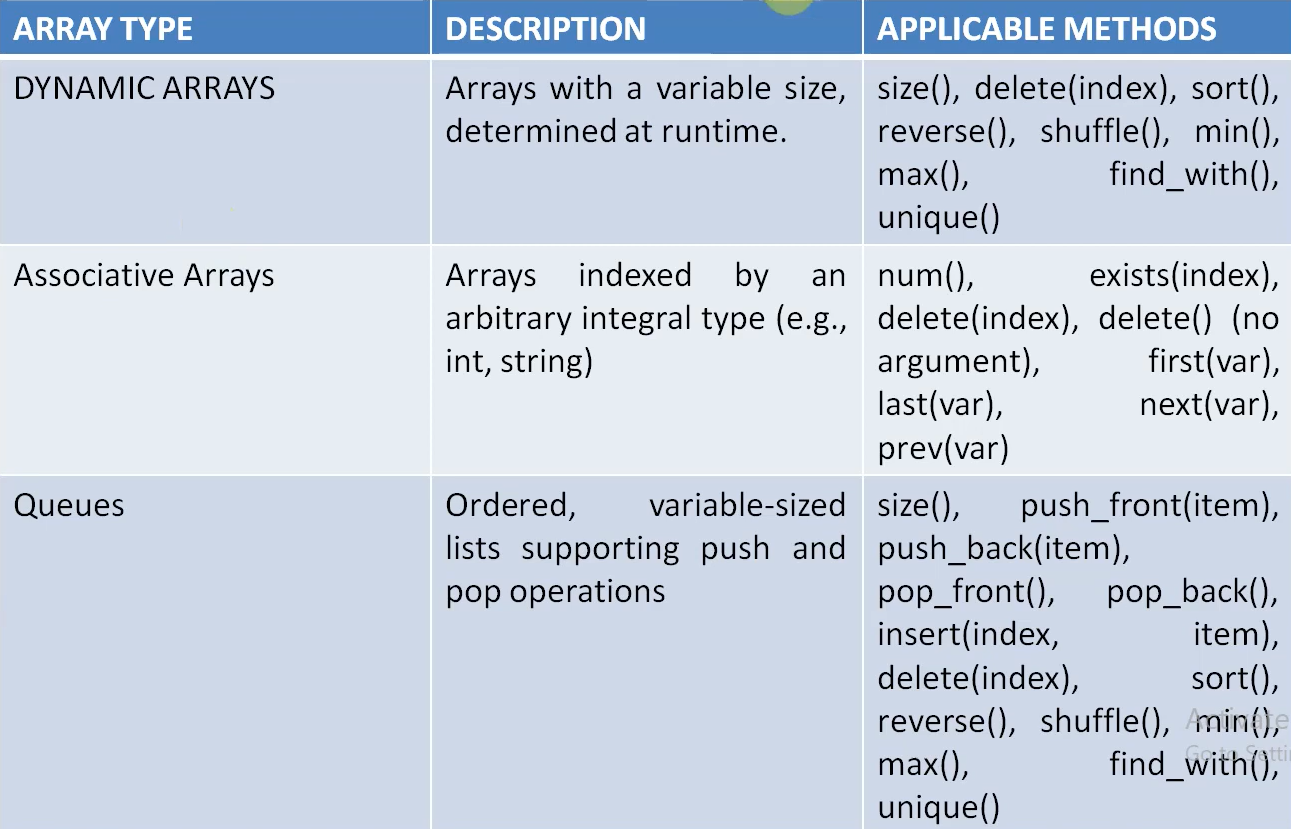
\includegraphics[width=0.8\textwidth]{DataTypes_sum1.png}
    % \caption{Summary of SystemVerilog Data Types}
    % \label{fig:data_types_summary}
\end{figure}
\vspace{-2em}
\begin{figure}[H]
    \centering
    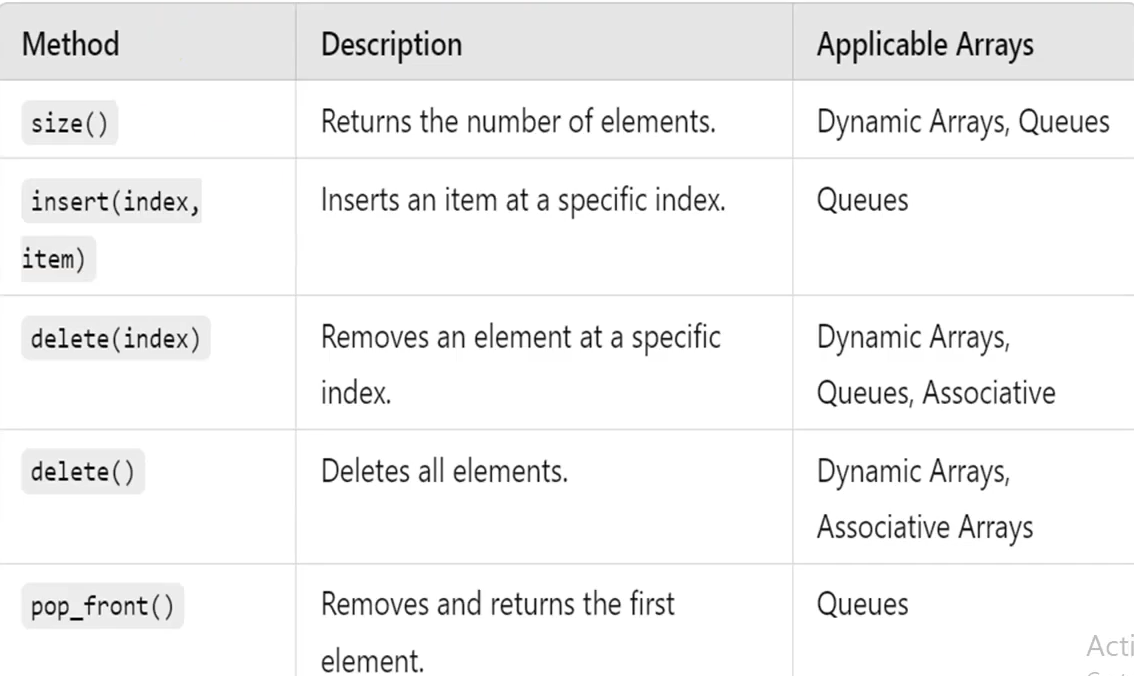
\includegraphics[width=0.8\textwidth]{DataTypes_sum2.png}
    % \caption{Summary of SystemVerilog Data Types (contd.)}
    % \label{fig:data_types_summary2}
\end{figure}
\vspace{-2em}
\begin{figure}[H]
    \centering
    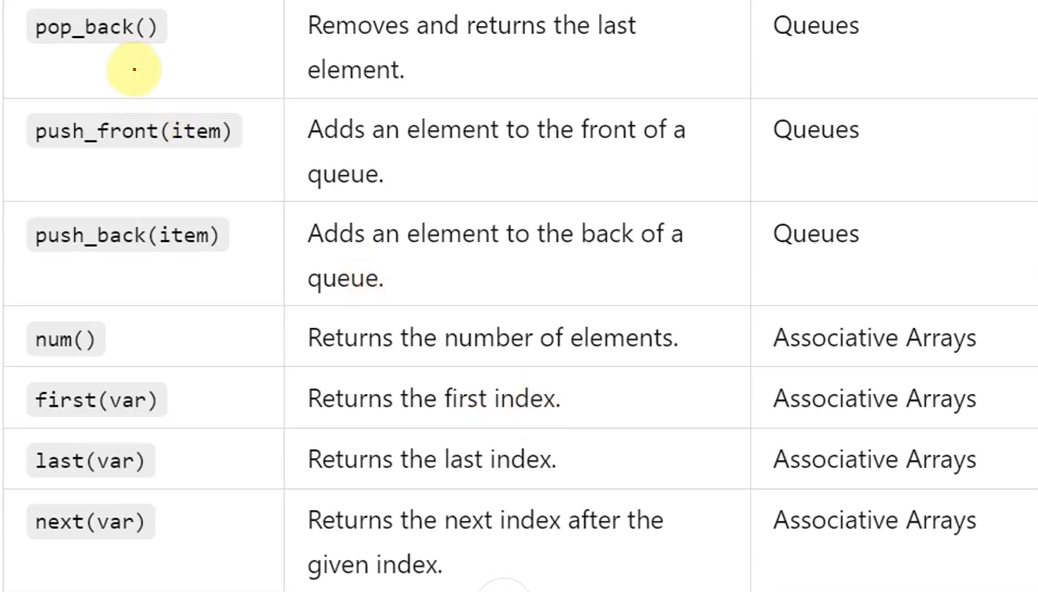
\includegraphics[width=0.8\textwidth]{DataTypes_sum3.png}
    % \caption{Summary of SystemVerilog Data Types (contd.)}
    % \label{fig:data_types_summary3}
\end{figure}
\vspace{-2em}
\begin{figure}[H]
    \centering
    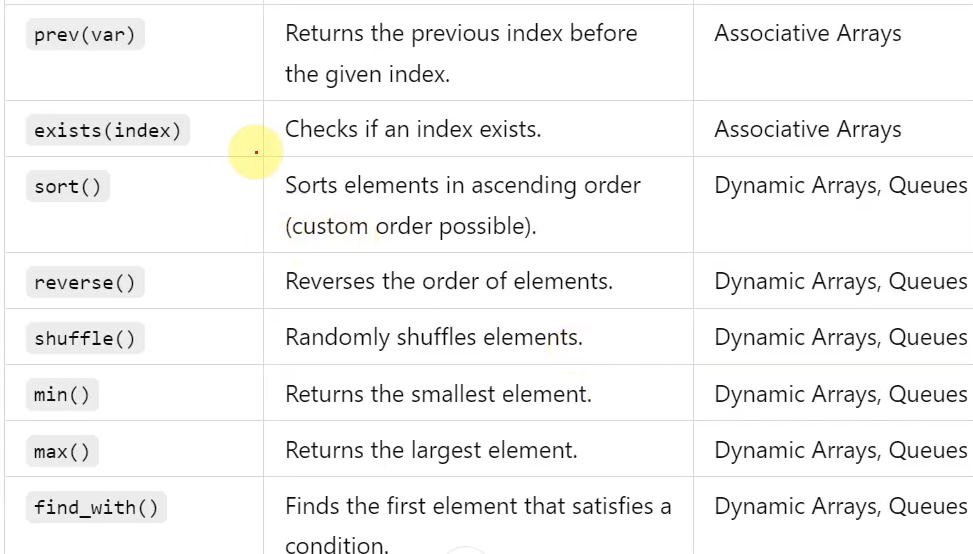
\includegraphics[width=0.8\textwidth]{DataTypes_sum4.png}
    % \caption{Summary of SystemVerilog Data Types (contd.)}
    % \label{fig:data_types_summary4}
\end{figure}

\subsection{Display Output}

In SystemVerilog, we can use the \texttt{\$display} function to print output to the console/Terminal. The \texttt{\$display} function is similar to the \texttt{printf} function in C/C++. It allows us to format the output and display variables, strings, and other data types.

\subsubsection{Format Specifiers}

The following table shows the format specifiers used with \texttt{\$display/\$write/\$monitor}  \texttt{/\$fwrite} in SystemVerilog:

\vspace{-1em}

\begin{center}
\begin{tabular}{|l|p{0.5\textwidth}|p{0.3\textwidth}|}
\hline
\textbf{Specifier} & \textbf{Meaning} & \textbf{Example Output} \\
\hline
\texttt{\%d} & Decimal (signed integer) & \texttt{42} \\
\hline
\texttt{\%0d} & Decimal with zero-padding (optional field width) & \texttt{00042} (if width is given) \\
\hline
\texttt{\%b} & Binary & \texttt{1010} \\
\hline
\texttt{\%h} & Hexadecimal & \texttt{A} \\
\hline
\texttt{\%o} & Octal & \texttt{12} \\
\hline
\texttt{\%c} & Character & \texttt{A} \\
\hline
\texttt{\%s} & String & \texttt{hello} \\
\hline
\texttt{\%p} & Aggregate (arrays, structs, etc.) & \texttt{'\{10, 20, 30\}} \\
\hline
\texttt{\%t} & Time (used in simulations) & \texttt{\#100} \\
\hline
\texttt{\%\%} & Prints a literal \texttt{\%} & \texttt{\%} \\
\hline
\end{tabular}
\end{center}

\textbf{Note:} The \texttt{\%p} format specifier is particularly useful for printing dynamic arrays, queues, associative arrays, and struct data types without needing to write explicit loops to display each element.

\subsubsection{Zero-Padding/Space-Padding}

In SystemVerilog, we can also specify the width of the output and whether to use zero-padding or space-padding. The following table summarizes the different formats:

\vspace{-0.8em}

\begin{center}
\begin{tabular}{|l|l|p{0.4\textwidth}|}
\hline
\textbf{Format} & \textbf{Name} & \textbf{Example Output (for x = 7)} \\
\hline
\texttt{\%0d} & Zero-padding (no width → acts like \texttt{\%d}) & \texttt{7} \textit{(no padding seen)} \\
\hline
\texttt{\%04d} & Zero-padding with width & \texttt{0007} \\
\hline
\texttt{\%4d} & Space-padding (right-aligned) & \texttt{   7} \textit{(3 spaces before 7)} \\
\hline
\texttt{\%-4d} & Left-aligned space-padding & \texttt{7   } \textit{(3 spaces after 7)} \\
\hline
\end{tabular}
\end{center}

\subsubsection{System Task}

Anything in verilog starting with \texttt{\$} is called a system task. System tasks are used to perform various operations such as displaying output, reading input, and controlling simulation time. Some commonly used system tasks are:

\begin{itemize}
    \item \texttt{\$display}: Used to display output to the console.
    \item \texttt{\$write}: Similar to \texttt{\$display}, but does not add a newline at the end of the output.
    \item \texttt{\$strobe}: 
    \item \texttt{\$monitor}: Used to monitor changes in signals and display output when a change occurs.
    \item \texttt{\$finish}: Used to terminate the simulation.
    \item \texttt{\$stop}: Used to pause the simulation.
    \item \texttt{\$time}: Returns the current simulation time.
\end{itemize}

\subsection{Tasks \& Functions}

In SystemVerilog, tasks and functions are procedural blocks that allows for executing a series of statements. Tasks are particularly useful when you need to group code that performs operations involving multiple inputs/outputs or when your code involves time-consuming operations (such as delays, waiting for an event, etc.). Tasks can be reused by calling them multiple times, helping to make your design more modular and easier to maintain.

Function is a subroutine that encapsulates reusable code and returns a single value. Functions are primarily used to perform calculations or operations that don't require simulation time, meaning they cannot contain any timing controls such as delays or event triggers.

\subsubsection{Enhancements in SystemVerilog:}

\begin{itemize}
    \item In Verilog, code inside task is guarded by \texttt{begin} and \texttt{end} keywords, while in SystemVerilog, no need to write these keywords.
    \item Function can only have input arguments in Verilog, while in SystemVerilog, it can have both input, inout and output arguments.
    \item We can't have void function in Verilog, while in SystemVerilog, we can have void function.
\end{itemize}

\textbf{Note:} SystemVerilog doesn't always support C-like inline initialization of local variables in task and function blocks — depending on tool and context. So it's safer to split declaration and assignment.

Example: \texttt{ int i = 10 + 20;} inside the task/function block will return i=0.

\subsubsection{Types of Tasks}

There are two types of tasks in SystemVerilog:
\begin{itemize}
    \item \textbf{Static Tasks:}
A static task in SystemVerilog is a task that does not maintain any state between invocations and shares its local variables across all calls. Static tasks are instantiated
once and their variables persist between calls, so changes made to variables in one invocation are visible in other invocations.

When the static task block is invokes/called for the first time, a memory space is allocated for the task and all member variables will be initialized. When it is called again, \ul{the same memory space is used} and the modification will be done in the same variables only.

By default, all tasks in SystemVerilog are static tasks. This means that if you don't specify otherwise, the task will behave as a static task.

\vspace{0.5em}
    \item \textbf{Automatic Tasks:}
A automatic task in SystemVerilog is a task that maintains its own state between invocations and does not share its local variables across calls. Automatic tasks are instantiated each time they are called, and their variables are initialized anew for each invocation.

When the automatic task block is invoked/called for the first time, a memory space is allocated for the task and all member variables will be initialized. \ul{The memory space is freed up when the task execution is completed}.

Everytime the automatic task is called, a \ul{new memory space is allocated} for the block of code and all member variables will be initialized again. This means that the automatic tasks does not retain any state between calls.

keyword \texttt{automatic} is used to declare a task as automatic.
\end{itemize}

\textbf{Important Note:} Static Task is better when the task is never recursive, never called in parallel, and performance is key, since automatic memory allocation has overhead. 
Automatic Task is preferred in case of multithreaded, or recursive use cases.

\subsubsection{Syntax of Task}

\begin{lstlisting}[
    language=Verilog,
    backgroundcolor={\color{gray!10}},
    numbers =none,
    % nolol=true,
    title={Static Task Syntax}
]
module task_example;

    int a;
    task increase();
        a=a+1;
    endtask

    task automatic increment();
        int i;
        i = i+1; // can't do int i = i+1;
        $display("The value of a after automatic increment is %0d", i);
    endtask

    initial begin
        increase();
        increment();
        $display("The value of a after 1st increment is %0d", a);
        
        increase();
        increment();
        $display("The value of a after 2nd increment is %0d", a);
    end
    
endmodule
\end{lstlisting}


\subsubsection{Passing arguments to Tasks}

In SystemVerilog, we can pass arguments to tasks in the following ways:
\begin{itemize}
    \item Argument passing by name
    
    \begin{lstlisting}[
        language=Verilog,
        backgroundcolor={\color{gray!10}},
        numbers =none,
        % nolol=true,
    ]
    task example_task(int a, int b);
        $display("The value of a is %0d and b is %0d", a, b);
    endtask
    initial begin
        example_task(.a(5), .b(10)); // Passing arguments by name
    end
    \end{lstlisting}

    \item Argument passing by value
    
    \begin{lstlisting}[
        language=Verilog,
        backgroundcolor={\color{gray!10}},
        numbers =none,
        % nolol=true,
    ]
    task example_task(int a, int b);
        $display("The value of a is %0d and b is %0d", a, b);
    endtask
    initial begin
        int x = 5;
        int y = 10;
        example_task(x, y); // Passing arguments by value
    end
    \end{lstlisting}
    
    \item Argument passing by reference
    
    Keyword \texttt{ref} is used to pass arguments by reference. This means that the task can modify the original variables passed to it, and those changes will be reflected outside the task. 
    
    The task must be declared automatic to use reference arguments. This is because passing by reference implies that the task or function can be re-entrant, meaning it can be called multiple times concurrently (or recursively), and each call needs its own independent set of local variables.

    \begin{lstlisting}[
        language=Verilog,
        backgroundcolor={\color{gray!10}},
        numbers =none,
        % nolol=true,
    ]
    task automatic example_task(ref int a, ref int b);
        a = a + 1;
        b = b + 2;
        $display("The value of a is %0d and b is %0d", a, b);
    endtask

    initial begin
        int x = 5;
        int y = 10;
        example_task(x, y); // Passing arguments by reference
        $display("The value of x after task call is %0d and y is %0d", x, y);
    end
    \end{lstlisting}

\end{itemize}

\textbf{Default Arguments}

\vspace{0.5em}

In SystemVerilog, we can also specify default values for task arguments. This allows us to call the task without providing all the arguments, and the default values will be used for any missing arguments.

\begin{lstlisting}[
    language=Verilog,
    backgroundcolor={\color{gray!10}},
    numbers =none,
    % nolol=true,
    title={Default Arguments in Task}
]
module task_example;

    task example_task(int a = 5, int b = 10);
        $display("The value of a is %0d and b is %0d", a, b);
    endtask

    initial begin
        example_task(); // Using default values
        example_task( , 20); // Using default value for b, leaving blank for a
        example_task(30, 40); // Using custom values
    end
endmodule
\end{lstlisting}

\subsection{Interface}

In SystemVerilog, an interface is a construct that allows you to group related signals and variables together, providing a way to define a common communication protocol between different modules.

\vspace{0.3em}

Lets say we are using the same set of signals in multiple modules, then instead of declaring the same signals in each module, we can declare them in an interface and use that interface in all the modules. This helps to reduce code duplication and makes the design more modular and easier to maintain.

\subsubsection{Syntax of Interface}
\begin{lstlisting}[
    language=Verilog,
    backgroundcolor={\color{gray!10}},
    numbers =none,
    % nolol=true,
    title={Interface Syntax}
]
interface my_if();
  int a;
  int b;
endinterface

// Here, I have declared the interface of two signals. This means that if I want to use these signals in any module then I can just create a instance of this inferface and include it directly.

module add(my_if intf);
  initial begin
    $display("sum is %0d", intf.a + intf.b);
  end
endmodule

module sub(my_if intf);
  initial begin
    $display("sum is %0d", intf.a - intf.b);
  end
endmodule

module operation;
  my_if intf();
  //   my_if is the interface name
  //  intf is the interface instance
  
    initial begin
        intf.a= 3;
 	 	intf.b= 4;
    end

  add adder(.intf(intf));
  sub subtrator(.intf(intf));
endmodule
\end{lstlisting}

We can pass any argument to the interface instance, it will be helpful in putting conditioning for the inputs signals. For example, if we want the signals to change with clock edge, then we can pass the clock signal to the interface instance and use it in the modules to modify the signals.
\begin{lstlisting}[
    language=Verilog,
    backgroundcolor={\color{gray!10}},
    numbers=none,
    % nolol=true,
    title={Interface with Clock Signal}
]
interface my_if(input logic clk);
  logic [7:0] data;
  logic valid;

  // Clocked process to update data and valid signals
  always_ff @(posedge clk) begin
    data <= data + 1; // Increment data on clock edge
    valid <= (data < 255); // Set valid based on data value
  end
endinterface

\end{lstlisting}

\subsubsection{Modports}

Modports (short for module ports) are a feature in SystemVerilog interfaces that allow you to define different access permissions rules (read/write directions) for the signals within the interface. It tells which signals are inputs, outputs, or inouts for a specific module using that interface.

\vspace{0.3em}

When multiple modules connect through the same interface, they may use the interface differently:

\begin{itemize}[nosep]
    \item One module might need to write to a signal, while another module might only need to read from it.
    \item One module might drive the signals (output). Another module might read the same signals (input).
\end{itemize}

\vspace{0.3em}

So, we use modport to define how each module can access the interface signals.

\begin{lstlisting}[
    language=Verilog,
    backgroundcolor={\color{gray!10}},
    numbers =none,
    % nolol=true,
    title={Modports in Interface}
]
 interface inf();
     int a;
     int b;
     int c;
     int d;
     
     modport master(input a, input b, output c);
     modport slave(input a, input b, input c, output d);
 endinterface
 
 module add_two(inf.master infc);
     assign infc.c = infc.a + infc.b;
 endmodule
 
 module add_three(inf.slave infc);
     assign infc.d = infc.a + infc.b + infc.c;
 endmodule
 
 module example_mud();
     inf my_inf();
     
     initial begin
         my_inf.a = 1;
         my_inf.b = 2;
     end
     
     add_two add1(my_inf); // same as add_two add1(.inf (my_inf))
     add_three add2(my_inf);
     
     initial begin
         #1;
         $display("The value of a and b is %0d, %0d",my_inf.c, my_inf.d);
     end
 endmodule
\end{lstlisting}

\subsection{Blocking \& Non-Blocking Assignments}

In Verilog, there are two types of assignments: blocking and non-blocking.

\begin{itemize}
    \item \textbf{Blocking assignments} (using the `=` operator) are executed sequentially. The next statement will not execute until the current statement is complete. This is similar to how assignments work in most programming languages.
    \item \textbf{Non-blocking assignments} (using the `<=` operator) allow the next statement to execute without waiting for the current statement to complete. This is useful in sequential logic, where you want to model flip-flops and other memory elements.
\end{itemize}

\subsubsection{Delay-Based Timining Control}
In Verilog, we can use delay-based timing control to specify the time delay for the execution of a statement. This is done using the \texttt{'\#'} symbol followed by the time delay value. This can be done in two ways:

\begin{itemize}
    \item \textbf{Inter Assignment Delay:} This is used to specify the time delay for the execution of a statement. The statement will be executed after the specified time delay. \ul{The delay value is specified on the left hand side of the expression.}
    \item \textbf{Intra Assignment Delay:} This is used to specify the time delay for the execution of a statement within a blocking assignment. The RHS to LHS assignment happens after the specified time delay. \ul{The delay value is specified on the right hand side of the assignment operator.}
\end{itemize}

 For both cases, the delay is specified in time units (e.g., nanoseconds, picoseconds, etc.) which is mentioned in the timescale directive at the top of the Verilog file.

\vspace{0.5em}

\textbf{Example-1:}

\begin{lstlisting}[
    language=Verilog,
    backgroundcolor={\color{gray!10}},
    numbers =none,
    % nolol=true,
        title={Delay-Based Timing Control}
    ]
        // Inter                     |          // Intra
     initial begin                   |          initial begin
        #10 b = 1;                   |              c = #10 a + b;
        #5 c = 5;                    |              d = #5 3;
    end                              |          end
\end{lstlisting}

In the above example, in case of inter assignment delay, the value of \texttt{b} will be assigned after 10 time units, and the value of \texttt{c} will be assigned after 15 time units (10 + 5). In case of intra assignment delay, the value of \texttt{c} will be assigned after 10 time units but the value of \texttt{a + b} will be evaluated at time = 0 only. The value of \texttt{d} will be assigned after 15 time units (10 + 5).

\vspace{1em}

\textbf{Example-2:}

\begin{lstlisting}[
    language=Verilog,
    backgroundcolor={\color{gray!10}},
    numbers =none,
    % nolol=true,
        title={Inter Assignment Delay in Non-Blocking Assignments}
    ]
        // Case-1        |        // Case-2           |       // Case-3
     initial begin       |      initial begin         |     initial begin
        a <= 0;          |          a <= 1;           |        a <= 1;
        b <= 1;          |          #5 b <= a + 1;    |        b <= #5 a + 1;
        c <= 2;          |          #10 c <= 3;       |        c <= #10 3;
        d <= 3;          |          #15 d <= 4;       |        d <= #15 4;
    end                  |      end                   |     end
\end{lstlisting}

\textbf{Case-1:}  This is simple non-blocking assignment execution. All the assignments will be executed in parallel and the values of \texttt{a}, \texttt{b}, \texttt{c}, and \texttt{d} will be 0, 1, 2, and 3 respectively at time t = 0. 

\vspace{0.2em}

\textbf{Case-2:}  Even though we are using the non-blocking assignments, this will be executed similar to blocking assignments because of inter assignment delays.
The assignments to \texttt{b}, \texttt{c}, and \texttt{d} have delays specified. The value of \texttt{b} will be assigned after 5 time units, \texttt{c} after 15 time units, and \texttt{d} after 30 (5+10+15) time units. The values of \texttt{a}, \texttt{b}, \texttt{c}, and \texttt{d} will still be 1, 2, 3, and 4 respectively after the execution of the initial block.

\vspace{0.2em}

\textbf{Case-3:}  In this case, the assignments to \texttt{b}, \texttt{c}, and \texttt{d} have delays specified. The value of \texttt{b} will be assigned after 5 time units, \texttt{c} after 10 time units, and \texttt{d} after 15 time units. However, the values of \texttt{a}, \texttt{b}, \texttt{c}, and \texttt{d} will be 1, 1, 3, and 4 respectively. Here, the value of \texttt{b} is different from Case-2 assigned after 5 time units, but the value of \texttt{a + 1} is evaluated at time t = 0 only. So, at time t=0, the value of \texttt{a} = 0, so the value of \texttt{b} will become 1. 


\textbf{Example-3:}

\begin{lstlisting}[
    language=Verilog,
    backgroundcolor={\color{gray!10}},
    numbers =none,
    % nolol=true,
        title={Intra Assignment Delay in Non-Blocking Assignments}
    ]  
     initial begin  
        a <= 0;       
        b <= #5 1;   
        c = #10 2;   
        d <= #3 3;
        e <= #5 4;    
    end                
\end{lstlisting}

Here, the value of  \texttt{a}, \texttt{b}, \texttt{c}, will be assigned after 0, 5, 10 time units respectively. The c statement will block the execution of further statements until it is executed completely. So, the value of \texttt{d} and \texttt{e} will be assigned after 13 time units (10 + 3) and 15 time units (10 + 5) respectively.

\subsection{Event Scheduler}

\href{http://www.sunburst-design.com/papers/CummingsSNUG2006Boston_SystemVerilog_Events.pdf}{Event Scheduler Paper}

\subsubsection{Simulation Time \& Time Slot}

In SystemVerilog, simulation time is divided into discrete time slots. Each time slot represents a specific point in time during the simulation. 
Time slot = all events processed at a single simulation time.

\begin{figure}[H]
    \centering
    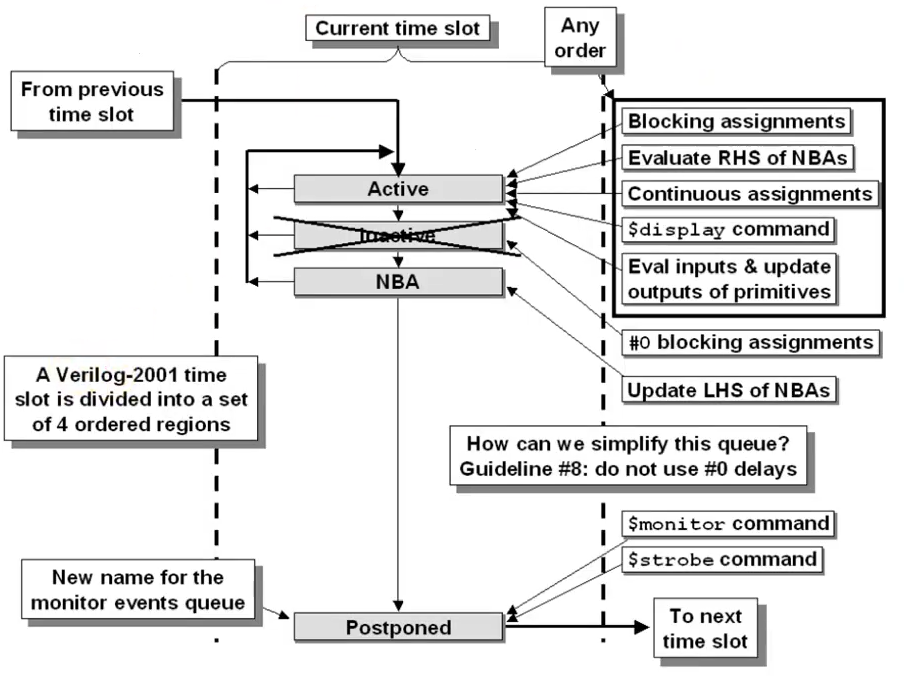
\includegraphics[width=0.8\textwidth]{Verilog_Event_Scheduler.png}
    \caption{Event Scheduler in Verilog}
    \label{fig:event_scheduler}
\end{figure}

To improve the the racing conditions, SystemVerilog introduces five more evnet regions in each time slot as shown below:

\begin{figure}[H]
    \centering
    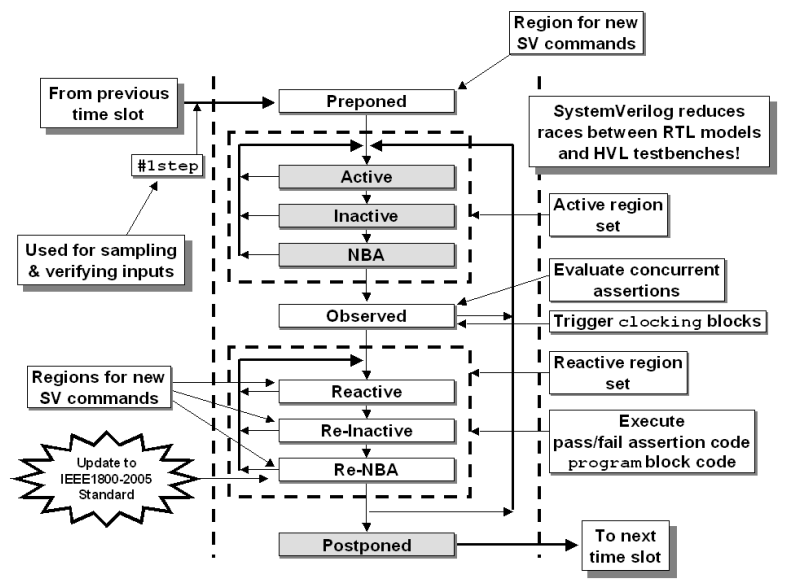
\includegraphics[width=0.8\textwidth]{SystemVerilog_Event_Scheduler.png}
    \caption{Event Scheduler in SystemVerilog}
    \label{fig:event_scheduler_sv}
\end{figure}

Simulation time moves in time slots, but within a time slot, a lot happens in steps (Preponed → Active → Inactive → NBA → Observed...).

\vspace{0.5em}

\textbf{Preponed Region}

The Preponed region happens first in a time slot, right after advancing simulation time, before anything else happens.

The Preponed region is read-only, meaning it doesn't change any signal values. Its \ul{main purpose is to capture (sample) signal values} for assertions before any updates or evaluations start.

This allows the testbench to capture the last known values before any design changes are applied.

\vspace{0.5em}

\textbf{Active Events Region}

The principal function of this region is to evaluate and execute all current module activity. There is no role of testbench in this region.
 
\begin{itemize}[nosep]
    \item Execute all \texttt{module} blocking assignments.
    \item Evaluate the Right-Hand-Side (RHS) of all nonblocking assignments and schedule updates into the NBA region.
    \item Execute all \texttt{module} continuous assignments
    \item Evaluate inputs and update outputs of Verilog primitives.
    \item Execute the \texttt{\$display} and \texttt{\$finish} commands.
\end{itemize}

\vspace{0.5em}
\textbf{Inactive Events Region}

\href{https://chatgpt.com/s/t_6860e9b687108191af38e7e5cd53e6ea}{ChatGPT Chat} for more details.

\vspace{0.5em}
\textbf{Non-Blocking Assignments (NBA) Region}

The principal function of this region is to execute the updates to the LeftHand-Side (LHS) variables that were scheduled in the Active region for all currently executing nonblocking assignments.

\vspace{0.5em}
\textbf{Observed Region}

The principal function of this region is to evaluate the concurrent assertions using the values sampled in the Preponed region.

\vspace{0.5em}
\textbf{Reactive Region Set}

This is a set dual of the corresponding Active regions. The Reactive region is used to run the testbench code, which is not part of the design under test (DUT), allowing the testbench to respond to the design events that happened earlier in the same time slot.

\vspace{0.5em}
\textbf{Postponed Region}

The principal function of this region is to execute the \texttt{\$strobe} and \texttt{\$monitor} commands that will show the final updated values for the current time slot.

\section{CVA6}

\textbf{References}: \href{https://github.com/openhwgroup/cva6}{GitHub Repository} \&
\href{https://github.com/VedantPahariya/cva6/blob/master/tutorials/running_sim.md}{Setup Tutorial} 

\textbf{Official Documentations} : \href{https://docs.openhwgroup.org/projects/cva6-user-manual/03_cva6_design/index.html}{CVA6 User Manual} \&
\href{https://cva6.readthedocs.io/en/latest/03_cva6_design/intro.html}{Main Theory}

\textbf{CVA6 GitHub Lab} : \href{https://github.com/sifferman/labs-with-cva6}{Hands-on-Experience with CVA6}

\vspace{0.4em}

\begin{figure}[h]
    \centering
    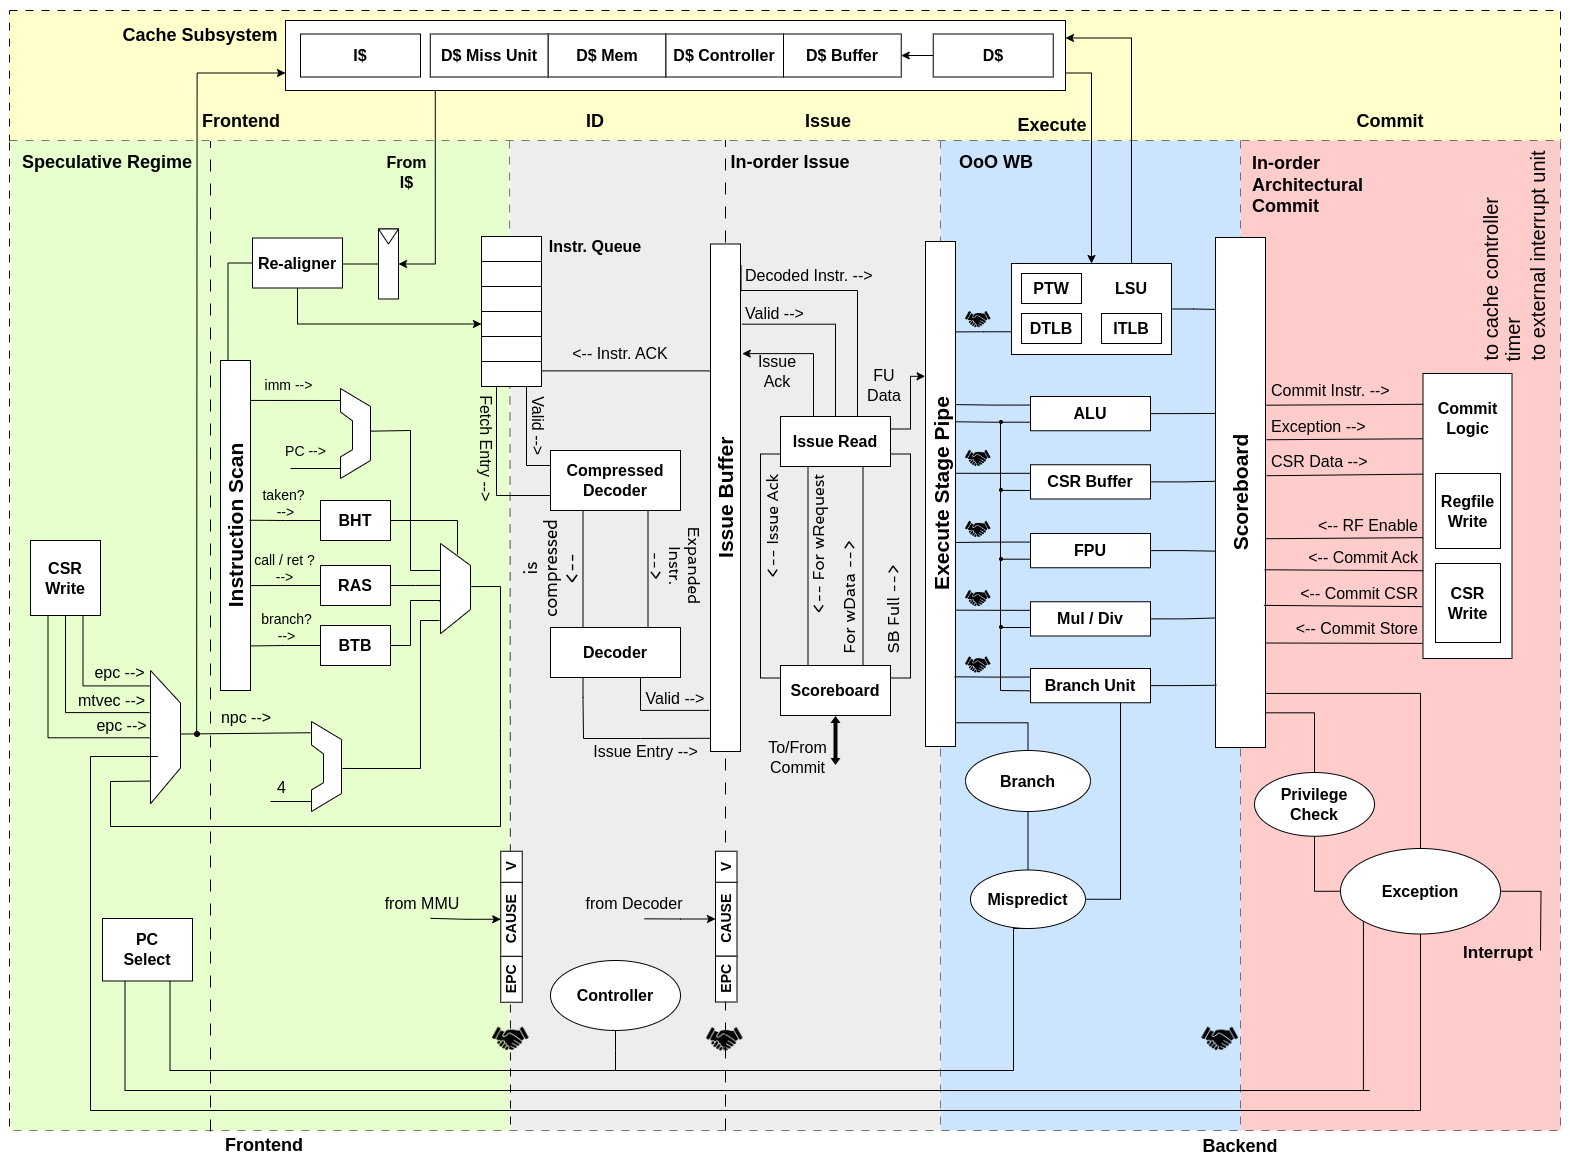
\includegraphics[width=1\textwidth]{CVA6.png}
    \caption{CVA6 Architecture}
    \label{fig:cva6_architecture}
\end{figure}    

CVA6 stands for CORE-V version of Ariane Core, which is a RISC-V based open-source processor core developed by the OpenHW Group. It is a 6-stage, single-issue, in-order CPU which implements the 64-bit RISC-V instruction set.

\vspace{0.4em}

\textbf{Note:} CVA6 is an in-order processor, which is true in the sense that instruction issue and commit happen in program order. However, its write-back and execution complete out-of-order. Click \href{https://chatgpt.com/s/t_6859b47774988191b23e0e92336e7668}{Here} for details (ChatGPT chat with sources).

\vspace{0.4em}

CVA6 supports I, M, A, and C extensions in RISC-V. \href{https://chatgpt.com/s/t_6859b7c99a1481919e4f0061d34eb39e}{Extracted details from Manual} (GPT) \& \href{https://www2.eecs.berkeley.edu/Pubs/TechRpts/2016/EECS-2016-118.pdf}{RISC-V Instruction Set Manual}

\vspace{0.4em}

It implements three privilege levels M, S, U to fully support a Unix-like operating system.
\href{https://chatgpt.com/s/t_6859b8e04be88191863e1d50b57d0f11}{GPT chat} for more details.

\subsection{Setting up CVA6}

To set up CVA6, you need to follow these steps:
\begin{enumerate}
    \item Fork the CVA6 repository and then clone from GitHub. \\
    Don't clone directly from the main repository, as it will not allow you to push changes (contribute back) in the future.

    \item Set upstream for pull the latest update

    \begin{lstlisting}[language=bash, frame=single, basicstyle=\ttfamily\footnotesize, numbers = none]
    git remote add upstream https://github.com/openhwgroup/cva6.git
    git remote -v
        \end{lstlisting}



    \item Initialize and update all submodules:

        \begin{lstlisting}[language=bash, frame=single, basicstyle=\ttfamily\footnotesize, numbers = none]
    git submodule update --init --recursive
        \end{lstlisting}

        Running this commmand ensures all submodules inside \hl{.gitmodules} —down to the deepest nested level—are initialized, cloned, and checked out to the exact commit expected by the main project. It's required to build and simulate complex repos like CVA6 smoothly. \href{https://chatgpt.com/s/t_6859c638d5208191bfd8707c9580f31a}{Link}
    
    \item Install cmake using following command:

        \begin{lstlisting}[language=bash, frame=single, basicstyle=\ttfamily\footnotesize, numbers =none]
    sudo apt install cmake
    cmake --version
        \end{lstlisting}

    \item Building the compiler Toolchain (\href{https://chatgpt.com/s/t_685e68ba0bfc81918b7b5a289666f145}{Steps})
        
        \href{https://chatgpt.com/s/t_685e51d3aca08191a9d3c16adf555498}{Why \& What Toolchain?} 

        Several standard packages are required to build the compiler toolchain. You can install them using the following command:

        \begin{lstlisting}[language=bash, frame=single, basicstyle=\ttfamily\footnotesize, numbers = none]
    sudo apt-get install autoconf automake autotools-dev curl git libmpc-dev libmpfr-dev libgmp-dev gawk build-essential bison flex texinfo gperf libtool bc zlib1g-dev
        \end{lstlisting}

        Under the \hl{\texttt{cva6/util/toolchain-builder/config}}, we have different toolchain configurations for different RISC-V targets.

        To build the specific toolchain, you can run the following command:

        \begin{lstlisting}[language=bash, frame=single, basicstyle=\ttfamily\footnotesize, numbers = none]
        bash get-toolchain.sh gcc-13.1.0-baremetal
        \end{lstlisting}

        The important step here is to set the configuration file 
        
        https://chatgpt.com/share/685e9b22-605c-8005-ad4d-3c5d990b4081

        \begin{lstlisting}[language=bash, frame=single, basicstyle=\ttfamily\footnotesize, numbers = none]
        export RISCV=$HOME/riscv
        export NUM_JOBS= 8
        ./build-toolchain.sh -f gcc-13.1.0-baremetal $RISCV
        \end{lstlisting}

        To check if it is installed correctly, you can run the following command:
        \begin{lstlisting}[language=bash, frame=single, basicstyle=\ttfamily\footnotesize, numbers = none]
        $HOME/riscv/bin/riscv-none-elf-gcc --version
            OR
        home/vedant/riscv/bin/riscv-none-elf-gcc --version
        \end{lstlisting}

\item Installing the Verilator and Spike
         \begin{lstlisting}[language=bash, frame=single, basicstyle=\ttfamily\footnotesize,numbers = none]
        export DV_SIMULATORS=veri-testharness,spike
        
        bash verif/regress/smoke-tests-cv64a6_imafdc_sv39.sh
         \end{lstlisting}

        Under CVA6/tools, we can clearly check two folders, spike and verilator-v5.008

        Run this to set them in path:
        
         \begin{lstlisting}[language=bash, frame=single, basicstyle=\ttfamily\footnotesize, numbers = none]
    export PATH=$(pwd)/tools/verilator-v5.008/bin:$(pwd)/tools/spike/bin:$PATH
    
    
    export PATH=/home/vedant/Desktop/Summer_Project/cva6/tools/spike/bin:$PATH
    export PATH=/home/vedant/Desktop/Summer_Project/cva6/tools/verilator-v5.008/bin:$PATH
    verilator --version
    spike --version
         \end{lstlisting}

         Then we can check the verilator and spike version.

    \item To run a C program, we can use the following code:

     \begin{lstlisting}[language=bash, 
 numbers = none, frame=single, basicstyle=\ttfamily\footnotesize]

 source verif/sim/setup-env.sh
 # run the above command in CVA6 directory
 
cd verif/sim

python3 cva6.py \
  --target cv64a6_imafdc_sv39 \
  --iss=veri-testharness \
  --iss_yaml=cva6.yaml \
  --c_tests ../tests/custom/hello_world/hello_world.c \
  --linker=../../config/gen_from_riscv_config/linker/link.ld \
  --gcc_opts="-static -mcmodel=medany -fvisibility=hidden -nostdlib \
  -nostartfiles -g ../tests/custom/common/syscalls.c \
  ../tests/custom/common/crt.S -lgcc \
  -I../tests/custom/env -I../tests/custom/common"
  \end{lstlisting}
\end{enumerate}

 \begin{lstlisting}[language=bash, 
 numbers = none, frame=single, basicstyle=\ttfamily\footnotesize]
 
export RISCV=$HOME/riscv
export RISCV_CC=/home/vedant/riscv/bin/riscv-none-elf-gcc
export SPIKE_PATH=/home/vedant/Desktop/Summer_Project/cva6/tools/spike/bin

\end{lstlisting}

Before running the below commands, run the above lines.



% Output directory
 % /home/vedant/Desktop/Summer_Project/cva6/verif/sim/out_2025-06-30
 
For converting .c file into .elf file:
\begin{lstlisting}[language=bash, frame=single, basicstyle=\ttfamily\footnotesize, numbers = none]
  export PATH=$HOME/riscv/bin:$PATH
  riscv-none-elf-gcc --version
  riscv-none-elf-gcc -o hello1.elf hello.c 
  # run this command where hello.c is present
 \end{lstlisting}

\begin{lstlisting}[language=bash, frame=single, basicstyle=\ttfamily\footnotesize, numbers = none]

/home/vedant/riscv/bin/riscv-none-elf-gcc \
verif/tests/custom/mytest/hello.c \
-T config/gen_from_riscv_config/linker/link.ld \
-static -mcmodel=medany -fvisibility=hidden -nostdlib -nostartfiles \
-g verif/tests/custom/common/syscalls.c verif/tests/custom/common/crt.S -lgcc \
-Iverif/tests/custom/env -Iverif/tests/custom/common -Iverif/env/p \
-o verif/sim/out_2025-07-03/directed_tests/hello.elf \
-march=rv64gc -mabi=lp64
 \end{lstlisting}

 Run the above command from CVA6 repo
 
 \url{https://chatgpt.com/s/t_6862946b5dbc81919ee5c69cf3d0d9a6}


Run all the setup here
\begin{lstlisting}[language=bash, frame=single, basicstyle=\ttfamily\footnotesize, numbers = none]
  export RISCV=$HOME/riscv
  source setup-env.sh  # run this in CVA6/verif/sim
  export NUM_JOBS=8
  export DV_SIMULATORS=veri-testharness,spike
  
    python3 cva6.py \
    --target cv64a6_imafdc_sv39 \
    --iss=$DV_SIMULATORS \
    --iss_yaml=cva6.yaml \
    --c_tests ../tests/custom/hello_world/hello_world.c \
    --linker=../../config/gen_from_riscv_config/linker/link.ld \
    --gcc_opts="-static -mcmodel=medany -fvisibility=hidden -nostdlib \
    -nostartfiles -g ../tests/custom/common/syscalls.c \
    ../tests/custom/common/crt.S -lgcc \
    -I../tests/custom/env -I../tests/custom/common"

 \end{lstlisting}


For waveform generation, use the following code:

\href{https://github.com/openhwgroup/cva6/blob/e34c5ba68358b26dfe13d0b953e622f2e9f8bebd/tutorials/running_sim.md?plain=1#L91-L123}{GitHub Official Instructions}

\begin{lstlisting}[language=bash, frame=single, basicstyle=\ttfamily\footnotesize, numbers = none]
    export TRACE_FAST=1
    export TRACE_COMPACT=1
\end{lstlisting}

\subsection{Stages in CVA6}

There are 6 stages in CVA6, which are as follows:

\begin{itemize}
    \item \textbf{PC generation Stage}: The Program Counter (PC) is generated to point to the next instruction to be executed.
    \item \textbf{Instruction Fetch Stage}: The instruction is fetched from memory.
    \item \textbf{Instruction Decode Stage}: The fetched instruction is decoded to determine the operation.
    \item \textbf{Issue Stage}: The instruction is issued to the appropriate execution unit.
    \item \textbf{Execute Stage}: The operation is performed (e.g., ALU operations, memory access).
    \item \textbf{Commit Stage}: The instruction is committed, and the next instruction is fetched.
\end{itemize}

\begin{figure}[h]
    \centering
    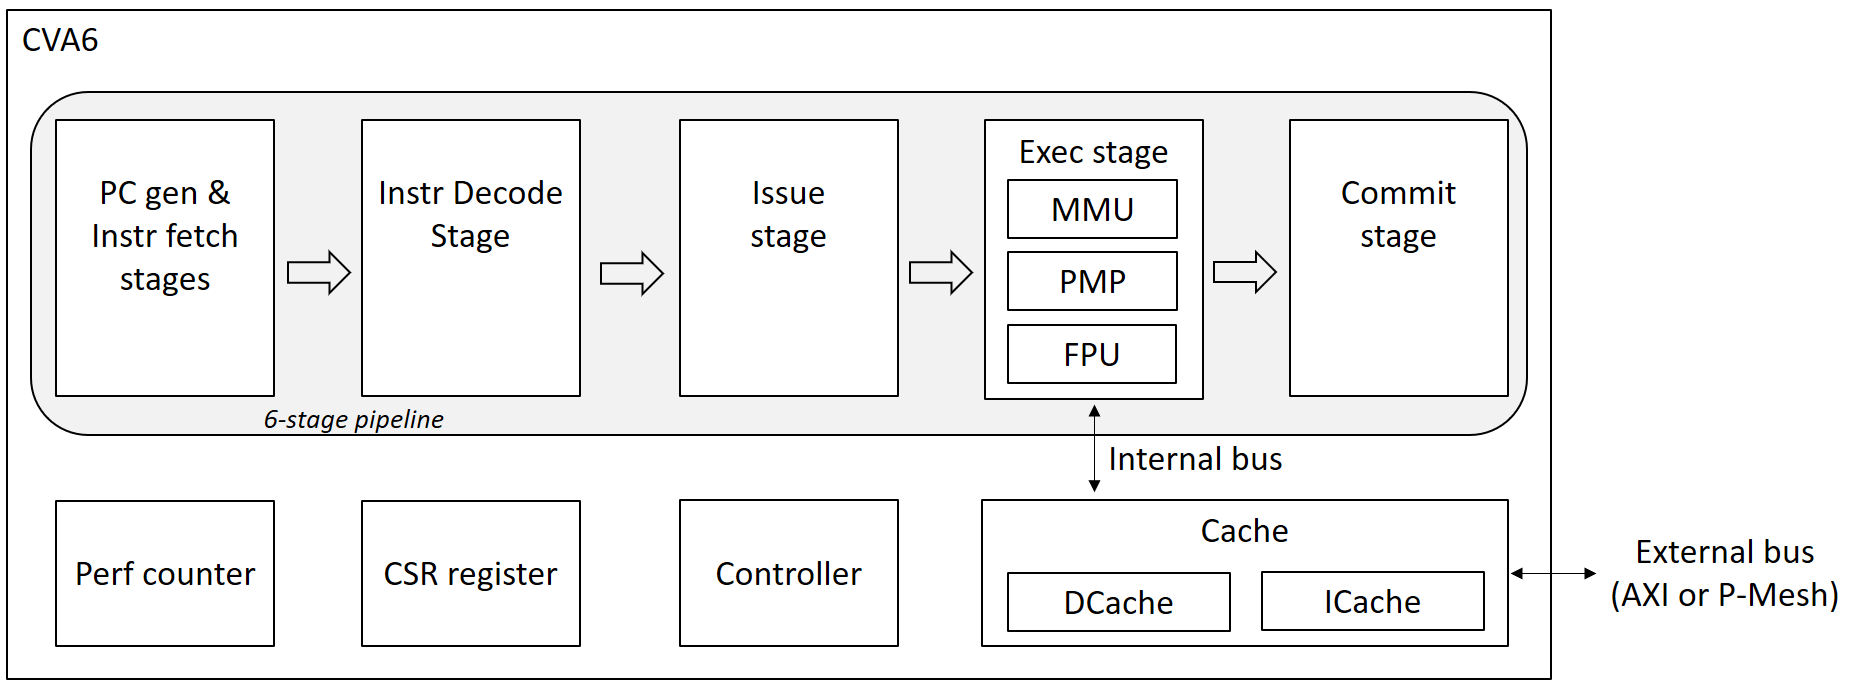
\includegraphics[width=0.8\textwidth]{CVA6_Stages.png}
    \caption{Stages in CVA6}
    \label{fig:cva6_stages}
\end{figure}

\subsubsection{PC generation Stage}

\vspace{0.5em}

The Instruction Cache (\$I) has 1 cycle access latency on hit while Data Cache (\$D) has longer latency of 3 cycles access latency on hit.

This stage is part of the frontend which includes branch prediction structures like BTB (Branch Target Buffer) and BHT (Branch History Table). The PC is generated based on the current PC value, branch prediction, and instruction fetch. 

\vspace{0.5em}

\textbf{Control and Status Register (CSR)}

These are the special registers which tell the CPU where to jump for special events (errors, OS calls, debug) by providing the addresses for exception/interrupt handling, environment call returns, and debug entry. and where to return after handling them, ensuring correct control flow in all situations (ensuring correct PC selection during exceptional control flow events).

\vspace{0.5em}

\subsubsection{Instruction Fetch Stage}

In this stage, the instruction is fetched from the instruction cache (\$I) based on the generated PC based on the handshake between the Instruction Fetch Unit (IFU) and the Instruction Cache. 

\vspace{0.5em}

The handshake is a classic "valid/ready" protocol:
\begin{itemize}[nosep]
    \item The frontend sets \texttt{icache\_dreq\_o.req} high when it wants to fetch an instruction.
    \item The instruction cache sets \texttt{icache\_dreq\_i.ready} high when it can accept a fetch request.
    \item Only when both signals are high in the same cycle does the fetch actually happen.
\end{itemize}


\textbf{Frontend wants to fetch:}
\begin{itemize}[nosep]
    \item \texttt{instr\_queue\_ready = 1} (queue has space)
    \item \texttt{halt\_frontend\_i = 0} (not halted)
    \item[$\rightarrow$] \texttt{icache\_dreq\_o.req = 1}
\end{itemize}

\textbf{Instruction cache is ready:}
\begin{itemize}[nosep]
    \item \texttt{icache\_dreq\_i.ready = 1}
\end{itemize}

\begin{lstlisting}[language=Verilog, frame=single, basicstyle=\ttfamily\footnotesize, numbers = none]
assign icache_dreq_o.req = instr_queue_ready & ~halt_frontend_i;
assign if_ready = icache_dreq_i.ready & instr_queue_ready & ~halt_frontend_i;
\end{lstlisting}

\begin{itemize}[nosep]
    \item \texttt{instr\_queue\_ready} ensures the instruction queue can accept new instructions.
    \item \texttt{halt\_frontend\_i} can block fetching (e.g., during a fence or halt).
\end{itemize}

\textbf{Fetch occurs:}
\begin{itemize}[nosep]
    \item \texttt{if\_ready = 1}
    \item The PC is updated, and the instruction cache returns the instruction data.
    \item If either side is not ready, the fetch is stalled until both are ready.
\end{itemize}

\vspace{0.5em}

\textbf{Why do we need an Instruction Cache and an Instruction Queue?}

\ul{Instruction Cache (I\$)}

It stores recently fetched instructions close to the CPU for fast access and reduces the need to access slow main memory for every instruction fetch.

Memory is much slower than the CPU. The cache bridges this speed gap, allowing the CPU to fetch instructions quickly and keep the pipeline full.

\ul{Instruction Queue}  

It buffers instructions fetched from the cache before they are sent to the decode stage and decouples the fetch stage from the decode/issue stages.

The instruction fetch and decode/issue stages may not always run at the same speed:
The cache might deliver multiple instructions at once (burst fetch).
The decode/issue stage might stall (e.g., due to pipeline hazards).
The queue allows the frontend to keep fetching instructions even if the backend is temporarily stalled, improving throughput and hiding memory/cache latency.

\vspace{0.5em}

\textbf{Branch Prediction}

Branch prediction data in CVA6 consists of:
\begin{itemize}[nosep]
    \item \textbf{BTB (Branch Target Buffer):} Remembers the target addresses of recently seen branches.
    \item \textbf{BHT (Branch History Table):} Remembers the recent outcomes (taken/not taken) of branches, usually using a small counter.
    \item \textbf{Index:} Subset of bits from the PC used to select (index into) a particular entry in the BTB/BHT tables. It provides the fast lookup into these tables using part of the PC.
    \item \textbf{Tag:} Subset of higher-order bits from the PC stored with each entry to help distinguish between different branches that might map to the same table entry (to avoid aliasing).
\end{itemize}

\textbf{Note/Fact:} The last bit(s) of the PC is always zero because when fetching instructions, the hardware fetches in words (32 bits = 4 bytes). This means the PC used for fetching is always aligned to 4 bytes, so the lowest two bits are zero. 
Even if the instruction is compressed (16 bits), the PC is still aligned to 2 bytes, so the lowest bit is zero.

\subsubsection{Instruction Decode Stage}
Because of the compressed instructions, this stage gets little complicated. It consists of three main components:
\begin{itemize}[nosep]
    \item \textbf{Instruction Re-aligner:} Handles compressed (16-bit) and regular (32-bit) instructions alignment across cache line boundaries.
    \item \textbf{Compressed Decoder:} raw 32-bit instruction words are transformed into executable control structures called scoreboard entries
    \item \textbf{Decoder} Contains the CPU's registers, which are used to store intermediate values during execution.
\end{itemize}

\subsubsection{Issue Stage}




\subsection{Understanding Spike \& Verilator}

Spike is the official RISC-V instruction set simulator (ISS) developed by UC Berkeley and maintained by the RISC-V community. It is referred as a golden reference software model for RISC-V processors. 

\vspace{0.5em}

\textbf{Note:} It is pre-written C++ code that implements RISC-V instructions functionally. It is not a simulator in the sense of simulating hardware, but rather a software model that executes RISC-V instructions.

\vspace{0.5em}

It executes RISC-V binaries (.ELF) according to the ISA spec.Spike simulates an idealized RISC-V processor that follows only the ISA specification - it doesn't know or care about CVA6's specific design choices.

Spike is like a "reference answer key" for what any RISC-V processor should do functionally, while Verilator shows what YOUR specific CVA6 processor actually does!

\subsection{Scoreboard}

Scoreboard is a hardware structure that tracks which instructions are in-flight (issued but not yet completed), which registers are being written, and which instructions are waiting for data.

Memory (data RAM/cache) accesses can take several cycles. If the CPU waits (stalls) every time it needs data from memory, performance drops. If an instruction is waiting for data (e.g., a load from memory), but there are other instructions that do not depend on that data, the CPU can execute those independent instructions while waiting. This helps in hiding latency.

\subsection{Model on Hardware}

\href{https://chatgpt.com/share/686529ac-6b08-8005-98f3-5291aa6a2816}{Step by step instruction}

grep is a powerful command-line tool used in Unix-like operating systems, such as Linux and macOS, for searching text files based on patterns. It stands for "global regular expression print". grep searches for lines in files that match a specified pattern (which can be a simple string or a more complex regular expression) and then prints those matching lines to the console.

The RISC-V testing infrastructure (like Spike or the CVA6 test framework) checks the special memory-mapped variable tohost. This value is used to signal success or failure of the program to the simulator.
When program exits, the runtime writes the return value to tohost. If it is zero means success else failure.

\subsubsection{Tests in CVA6}

There are following tests like:

\begin{itemize}[nosep]
    \item \textbf{run-asm-tests}: Runs all RISC-V assembly tests (from ci/riscv-asm-tests.list).
    \item \textbf{run-amo-tests}: Runs atomic memory operation tests.
    \item \textbf{run-mul-tests}: Runs multiplication instruction tests.
    \item \textbf{run-fp-tests}: Runs floating-point instruction tests.
    \item \textbf{run-benchmarks}: Runs benchmark programs.
\end{itemize}

Each of these targets will simulate a suite of tests using the test lists defined in the ci/ directory.

To run a specific test, you can use the following command:
\begin{lstlisting}[language=bash, frame=single, basicstyle=\ttfamily\footnotesize, numbers = none]
   make run-mul-tests
\end{lstlisting}

\textbf{Log File Format:}

\begin{figure}[h]
    \centering
    \includegraphics[width=0.8\textwidth]{CVA6_log_file.png}
    \caption{CVA6 Log File Instructions}
    \label{fig:cva6_log_format}
\end{figure}

Each instruction is logged in two parts:
\begin{itemize}
  \item \textbf{Instruction Decode Line:}
  \begin{quote}
    \texttt{core   0: 0x0000000000010000 (0x00100413) li s0, 1}
  \end{quote}
  This shows that core 0 executed the instruction \texttt{li s0, 1} at address \texttt{0x0000000000010000} (PC Value), which has 32-bit RISC-V machine code (actual instruction) in Hex (\texttt{0x00100413}) stored at that address.

  \item \textbf{Writeback Line (if register is written):}
  \begin{quote}
    \texttt{3 0x0000000000010000 (0x00100413) x 8 0x0000000000000001}
  \end{quote}
  Here, the number \texttt{3} indicates Machine mode, register \texttt{x8} was updated with value \texttt{0x1}. PC and Instruction is repeated. There are other modes like \texttt{0} for User mode and \texttt{1} for Supervisor mode. The instruction was executed in Machine Mode, the highest privilege level in RISC-V.
\end{itemize}

Note: 
li s0, 1  $\rightarrow$ which is a pseudoinstruction for: addi s0, zero, 1

\subsection{Performance Modelling}

\subsubsection{RVFI Trace}

RVFI (RISC-V Formal Interface) trace is a standardized way to capture and analyze the execution of RISC-V instructions in a simulation environment. It records:

\begin{itemize}[nosep]
    \item Instruction execution
    \item Register updates
    \item Memory accesses
    \item Program Counter (PC) values
    \item Timing information
\end{itemize}

\vspace{0.5em}

\textbf{RVFI Analyser}

This is a script written by copilot to analyse the RVFI trace file generated by the CVA6 simulator. To run the script, You can run the script using the following command:

\begin{lstlisting}[language=bash, frame=single, basicstyle=\ttfamily, numbers=none]
   python3 rvfi_analyser.py <rvfi_trace_file>
\end{lstlisting}

Example:
\begin{lstlisting}[language=bash, frame=single, 
    basicstyle=\ttfamily, numbers=none]
python3 rvfi_analyzer.py \
verif/sim/out_2025-07-02/veri-testharness_sim/hello_world.cv64a6_imafdc_sv39.log
\end{lstlisting}      

There are four files for analysing log files:
\begin{itemize}
    \item \textbf{rvfi\_analyzer.py}: Instruction type distribution, proper log instruction printing
    \item \textbf{simple\_rvfi\_analyzer.py}: Simple analysis of RVFI traces
    \item \textbf{analysis.py}: Subset result of model.py. RVFI analysis for issue=commit=2
    \item \textbf{demo\_issue\_commit.py}: Issue and Commit width analysis with Hazard and Improvement Analysis. Varies the issue and commit width, put the data for each of them
    \item \textbf{model.py}: issue/commit matrix
\end{itemize}


\textbf{Complete Execution Flow}

This is python script to completely analyse the instructions

\begin{lstlisting}[language=bash, frame=single, basicstyle=\ttfamily\footnotesize, numbers=none]
python3 perf_analysis.py ../verif/sim/out_2025-07-08/veri-testharness_sim/multiply.cv64a6_imafdc_sv39.log --performance --save-terminal-output corrected_test.txt --colors
\end{lstlisting}

\textbf{Getting the Scoreboard Result\\}
For printing the scoreboard debug, run the following:

\begin{lstlisting}[language=bash, frame=single, basicstyle=\ttfamily\footnotesize, numbers=none]
python3 debug_model.py ../verif/sim/out_2025-07-08/veri-testharness_sim/multiply.cv64a6_imafdc_sv39.log

\end{lstlisting}

This will generate the output file \texttt{scoreboard\_debug\_\textless filename\textgreater.log} 

For removing files and checking memory space from Linux terminal:
https://chatgpt.com/share/688a6899-06f0-8005-aea7-fcab78d27963

\section{PULP-TrainLib}

\section{UVM}
Reference: \href{https://youtube.com/playlist?list=PLuYB6t6povcLgoHWLJgk-VeMQ0Rscjw03&si=l-rjyvLkuttomYeC}{Playlist1}
\href{https://youtube.com/playlist?list=PLqPfWwayuBvNrr09dCweog1htCBLUbN4W&si=4vI1Fs_sgz-A0wXdC}{Playlist2} are the links to the UVM playlists.

\section{On-Device Training}

% Basic Latex Template
\subsubsection{Subsection}

Introduce about the \underline{Title} here. \\

% Here is the way to attach the links in the document
Reference: \url{https://www.youtube.com/watch?v=ic1UMeuCBA8} \\
\href{https://www.geeksforgeeks.org/difference-between-gate-level-and-structural-verilog-hdl/}{GeeksforGeeks}

\begin{itemize}
    \item \textbf{1}: 
    \item \textbf{2}:   
\end{itemize}

\begin{figure}[h]   % h stands for here, t for top, b for bottom, p for page
    \centering
    \includegraphics[width=0.65\textwidth]{example-image-a} % width is in fraction of textwidth
    \caption{Sample Image}% Caption of the image
    \label{fig:veri1}
\end{figure}

Verilog is a \underline{Case Sensitive} language. \\
The term ``module'' refers to the text enclosed by the keyword pair \textbf{module} \ldots \textbf{endmodule}. Module is the fundamental descriptive unit in Verilog language. \\
Keyword ``module'' is followed by the \underline{name of the design} (ABC here) and \uline{parenthesis - enclosed list of ports}.\\
% uline works better than underline when the text is being wrapped and going in the next line. 

\end{document}